% Options for packages loaded elsewhere
\PassOptionsToPackage{unicode}{hyperref}
\PassOptionsToPackage{hyphens}{url}
\documentclass[
  10pt,
]{article}
\usepackage{xcolor}
\usepackage{amsmath,amssymb}
\setcounter{secnumdepth}{-\maxdimen} % remove section numbering
\usepackage{iftex}
\ifPDFTeX
  \usepackage[T1]{fontenc}
  \usepackage[utf8]{inputenc}
  \usepackage{textcomp} % provide euro and other symbols
\else % if luatex or xetex
  \usepackage{unicode-math} % this also loads fontspec
  \defaultfontfeatures{Scale=MatchLowercase}
  \defaultfontfeatures[\rmfamily]{Ligatures=TeX,Scale=1}
\fi
\usepackage{lmodern}
\ifPDFTeX\else
  % xetex/luatex font selection
  \setmainfont[]{Times New Roman}
  \setmonofont[]{Menlo}
\fi
% Use upquote if available, for straight quotes in verbatim environments
\IfFileExists{upquote.sty}{\usepackage{upquote}}{}
\IfFileExists{microtype.sty}{% use microtype if available
  \usepackage[]{microtype}
  \UseMicrotypeSet[protrusion]{basicmath} % disable protrusion for tt fonts
}{}
\makeatletter
\@ifundefined{KOMAClassName}{% if non-KOMA class
  \IfFileExists{parskip.sty}{%
    \usepackage{parskip}
  }{% else
    \setlength{\parindent}{0pt}
    \setlength{\parskip}{6pt plus 2pt minus 1pt}}
}{% if KOMA class
  \KOMAoptions{parskip=half}}
\makeatother
\usepackage{color}
\usepackage{fancyvrb}
\newcommand{\VerbBar}{|}
\newcommand{\VERB}{\Verb[commandchars=\\\{\}]}
\DefineVerbatimEnvironment{Highlighting}{Verbatim}{commandchars=\\\{\}}
% Add ',fontsize=\small' for more characters per line
\newenvironment{Shaded}{}{}
\newcommand{\AlertTok}[1]{\textcolor[rgb]{1.00,0.00,0.00}{\textbf{#1}}}
\newcommand{\AnnotationTok}[1]{\textcolor[rgb]{0.38,0.63,0.69}{\textbf{\textit{#1}}}}
\newcommand{\AttributeTok}[1]{\textcolor[rgb]{0.49,0.56,0.16}{#1}}
\newcommand{\BaseNTok}[1]{\textcolor[rgb]{0.25,0.63,0.44}{#1}}
\newcommand{\BuiltInTok}[1]{\textcolor[rgb]{0.00,0.50,0.00}{#1}}
\newcommand{\CharTok}[1]{\textcolor[rgb]{0.25,0.44,0.63}{#1}}
\newcommand{\CommentTok}[1]{\textcolor[rgb]{0.38,0.63,0.69}{\textit{#1}}}
\newcommand{\CommentVarTok}[1]{\textcolor[rgb]{0.38,0.63,0.69}{\textbf{\textit{#1}}}}
\newcommand{\ConstantTok}[1]{\textcolor[rgb]{0.53,0.00,0.00}{#1}}
\newcommand{\ControlFlowTok}[1]{\textcolor[rgb]{0.00,0.44,0.13}{\textbf{#1}}}
\newcommand{\DataTypeTok}[1]{\textcolor[rgb]{0.56,0.13,0.00}{#1}}
\newcommand{\DecValTok}[1]{\textcolor[rgb]{0.25,0.63,0.44}{#1}}
\newcommand{\DocumentationTok}[1]{\textcolor[rgb]{0.73,0.13,0.13}{\textit{#1}}}
\newcommand{\ErrorTok}[1]{\textcolor[rgb]{1.00,0.00,0.00}{\textbf{#1}}}
\newcommand{\ExtensionTok}[1]{#1}
\newcommand{\FloatTok}[1]{\textcolor[rgb]{0.25,0.63,0.44}{#1}}
\newcommand{\FunctionTok}[1]{\textcolor[rgb]{0.02,0.16,0.49}{#1}}
\newcommand{\ImportTok}[1]{\textcolor[rgb]{0.00,0.50,0.00}{\textbf{#1}}}
\newcommand{\InformationTok}[1]{\textcolor[rgb]{0.38,0.63,0.69}{\textbf{\textit{#1}}}}
\newcommand{\KeywordTok}[1]{\textcolor[rgb]{0.00,0.44,0.13}{\textbf{#1}}}
\newcommand{\NormalTok}[1]{#1}
\newcommand{\OperatorTok}[1]{\textcolor[rgb]{0.40,0.40,0.40}{#1}}
\newcommand{\OtherTok}[1]{\textcolor[rgb]{0.00,0.44,0.13}{#1}}
\newcommand{\PreprocessorTok}[1]{\textcolor[rgb]{0.74,0.48,0.00}{#1}}
\newcommand{\RegionMarkerTok}[1]{#1}
\newcommand{\SpecialCharTok}[1]{\textcolor[rgb]{0.25,0.44,0.63}{#1}}
\newcommand{\SpecialStringTok}[1]{\textcolor[rgb]{0.73,0.40,0.53}{#1}}
\newcommand{\StringTok}[1]{\textcolor[rgb]{0.25,0.44,0.63}{#1}}
\newcommand{\VariableTok}[1]{\textcolor[rgb]{0.10,0.09,0.49}{#1}}
\newcommand{\VerbatimStringTok}[1]{\textcolor[rgb]{0.25,0.44,0.63}{#1}}
\newcommand{\WarningTok}[1]{\textcolor[rgb]{0.38,0.63,0.69}{\textbf{\textit{#1}}}}
\usepackage{longtable,booktabs,array}
\usepackage{calc} % for calculating minipage widths
% Correct order of tables after \paragraph or \subparagraph
\usepackage{etoolbox}
\makeatletter
\patchcmd\longtable{\par}{\if@noskipsec\mbox{}\fi\par}{}{}
\makeatother
% Allow footnotes in longtable head/foot
\IfFileExists{footnotehyper.sty}{\usepackage{footnotehyper}}{\usepackage{footnote}}
\makesavenoteenv{longtable}
\usepackage{graphicx}
\makeatletter
\newsavebox\pandoc@box
\newcommand*\pandocbounded[1]{% scales image to fit in text height/width
  \sbox\pandoc@box{#1}%
  \Gscale@div\@tempa{\textheight}{\dimexpr\ht\pandoc@box+\dp\pandoc@box\relax}%
  \Gscale@div\@tempb{\linewidth}{\wd\pandoc@box}%
  \ifdim\@tempb\p@<\@tempa\p@\let\@tempa\@tempb\fi% select the smaller of both
  \ifdim\@tempa\p@<\p@\scalebox{\@tempa}{\usebox\pandoc@box}%
  \else\usebox{\pandoc@box}%
  \fi%
}
% Set default figure placement to htbp
\def\fps@figure{htbp}
\makeatother
\setlength{\emergencystretch}{3em} % prevent overfull lines
\providecommand{\tightlist}{%
  \setlength{\itemsep}{0pt}\setlength{\parskip}{0pt}}

% ICLR-style page: 5.5in text block on US letter, Times, 10pt
\usepackage[letterpaper,left=1.5in,right=1.5in,top=1in,bottom=1in]{geometry}
\usepackage{amsmath,amssymb,amsthm}
\usepackage{graphicx}
\usepackage{booktabs}
\usepackage{longtable}
\usepackage{array}
\usepackage{microtype}
\usepackage[table]{xcolor}
\usepackage{caption}
\usepackage{titlesec}
\usepackage{titling}
\usepackage[colorlinks=true,linkcolor=blue!45!black,urlcolor=blue!45!black,
            citecolor=blue!45!black]{hyperref}
\theoremstyle{plain}
\newtheorem{theorem}{Theorem}
\newtheorem{proposition}[theorem]{Proposition}
\newtheorem{corollary}[theorem]{Corollary}
\theoremstyle{definition}
\newtheorem{assumption}{Assumption}
\setlength{\emergencystretch}{3em}
\providecommand{\tightlist}{\setlength{\itemsep}{0pt}\setlength{\parskip}{0pt}}
\captionsetup{font=small,labelfont=bf}

\titleformat{\section}{\normalfont\large\bfseries}{\thesection}{0.7em}{}
\titleformat{\subsection}{\normalfont\normalsize\bfseries}{\thesubsection}{0.6em}{}
\titleformat{\subsubsection}{\normalfont\normalsize\bfseries\itshape}{\thesubsubsection}{0.6em}{}
\titlespacing*{\section}{0pt}{1.7ex plus .6ex minus .2ex}{1.0ex plus .2ex}
\titlespacing*{\subsection}{0pt}{1.3ex plus .5ex minus .2ex}{0.8ex plus .2ex}
\titlespacing*{\subsubsection}{0pt}{1.1ex plus .4ex minus .2ex}{0.7ex plus .2ex}

\pretitle{\begin{center}\LARGE\bfseries}
\posttitle{\par\end{center}\vskip 0.4em}
\preauthor{\begin{center}\large}
\postauthor{\par\end{center}}
\predate{\begin{center}\normalsize}
\postdate{\par\end{center}\vskip 0.8em}

\newenvironment{iclrabstract}
  {\vspace{0.4em}\begin{center}{\bfseries\scshape Abstract}\end{center}
   \begin{list}{}{\setlength{\leftmargin}{0.45in}\setlength{\rightmargin}{0.45in}}\item[]\relax}
  {\end{list}\vspace{0.6em}}

% wide tables and figures shrink to the measure instead of running off the page
\newcommand{\fitwidth}[1]{\makebox[\linewidth][c]{\resizebox{\ifdim\width>\linewidth\linewidth\else\width\fi}{!}{#1}}}

% Times carries no mathematical glyphs; give those code points a real font
\usepackage{newunicodechar}
\newfontfamily\symfont{STIX Two Math}[Scale=MatchLowercase]
\newunicodechar{ℝ}{{\symfont ℝ}}
\newunicodechar{ℙ}{{\symfont ℙ}}
\newunicodechar{𝔼}{{\symfont 𝔼}}
\newunicodechar{∈}{{\symfont ∈}}
\newunicodechar{⋃}{{\symfont ⋃}}
\newunicodechar{∪}{{\symfont ∪}}
\newunicodechar{⊆}{{\symfont ⊆}}
\newunicodechar{⊂}{{\symfont ⊂}}
\newunicodechar{∝}{{\symfont ∝}}
\newunicodechar{∎}{{\symfont ∎}}
\newunicodechar{≪}{{\symfont ≪}}
\newunicodechar{∼}{{\symfont ∼}}
\newunicodechar{∅}{{\symfont ∅}}
\newunicodechar{₉}{{\symfont ₉}}
\newunicodechar{₅}{{\symfont ₅}}
\newunicodechar{⁻}{{\symfont ⁻}}

\pagestyle{plain}
\setlength{\parskip}{0.45em}
\setlength{\parindent}{0pt}
\usepackage{bookmark}
\IfFileExists{xurl.sty}{\usepackage{xurl}}{} % add URL line breaks if available
\urlstyle{same}
\hypersetup{
  pdftitle={Proxy Embeddings: Why You Cannot Validate a Proxy by Correlating It With the Artifact},
  hidelinks,
  pdfcreator={LaTeX via pandoc}}

\title{Proxy Embeddings: Why You Cannot Validate a Proxy by Correlating
It With the Artifact}
\author{}
\date{}

\begin{document}
\maketitle

\begin{iclrabstract}

A synthetic-data pipeline embeds text and then acts on the distances:
drop the near-duplicates, keep the most different items, retrieve
neighbours, screen for contamination. Every one of those decisions bets
that proximity in the embedding stands in for proximity in the thing the
text becomes --- a program that runs, a query that returns rows, a
picture that gets rendered. The usual way to check the bet is to decode
a sample and report a correlation.

\textbf{That check does not work, and we can say exactly why.} On 553
generated Python programs decoded by execution on a fixed 140-input
battery, text distance and behavioural distance correlate at +0.451
among the closest decile of pairs and +0.065 among the farthest --- an
apparently sharp result saying that embeddings track behaviour among
near-duplicates and carry nothing beyond them. Running the identical
analysis between two \emph{encoders}, with no decoder anywhere, gives
\textbf{+0.742 to +0.781} for the same near-minus-far quantity:
\textbf{the decoder-free control shows the effect about twice as
strongly as the decoder does.} The conditional-mean curves coincide. The
shape is a property of comparing two distance matrices, not of the
artifact. A permutation null does flatten (−0.025), so a real
text-to-behaviour association exists; what does not exist is evidence
for the mechanism the profile appears to show.

This is the check the field runs when it proposes an embedding proxy for
something expensive, frequently with the observation that agreement is
strongest among similar items. We give the control that should accompany
it, and the positive alternative: \textbf{validate a proxy by running
the decision, not by correlating the distances.} Scored that way, on
decoders that are deterministic and total, three decisions come apart
cleanly.

\textbf{Deduplication is a corpus instrument, not an item gate.}
Duplicate-pair detection runs at AUC 0.779, but at the tightest radius
tested \textbf{45.4\% of the pairs a filter would reject are
behaviourally far apart} (41.6\% on a second decoder), so a filter
defensible for contamination screening is not defensible per item, and
no threshold fixes it.

\textbf{Diversity selection has no stable sign.} Greedy max-min loses to
random at every budget on one decoder and beats it from \emph{k} = 20 on
another. It cannot be predicted from the embedding and has to be
measured.

\textbf{Both signs lose to the artifact-space oracle, which is cheaper
than the proxy.} The oracle reaches at \emph{k} = 30 what the best
text-space selector needs \emph{k} = 100 to reach. Decoding a generated
program in its own operating-system process costs 29.1 ms against 107.9
ms for a batched local embedding; tracing an \texttt{ipaddress} call
costs 0.98 ms against 685 ms. For deterministic decoders the oracle is
not the option a practitioner cannot afford but the one they did not
think to run.

Text-level deduplication performed perfectly on this corpus removes 63\%
of it and leaves it \textbf{5.2× redundant in the space that matters}:
203 distinct programs, 39 distinct behaviours.

We ship all of it as \texttt{decodergap}, which reports the decoder-free
control beside every correlation and scores each decision in the
artifact\textquotesingle s own space. Alongside this we report the same
question where decoding is genuinely expensive --- rendered images and
audio --- where text-embedding similarity explains 14.5\% of the
variance in rendered-image similarity, whether a prompt can be steered
at all is a property of the embedder, and a third of the conditioning is
lost at the seam where one model\textquotesingle s language becomes
another model\textquotesingle s input.

\begin{center}\rule{0.5\linewidth}{0.5pt}\end{center}

\end{iclrabstract}

\subsection{1. Introduction}\label{1-introduction}

A generated corpus is almost never the thing anyone wants. It is a step
towards the thing: the program that will run, the query that will return
rows, the picture that will be rendered, the model that will be
fine-tuned. Between the text and the artifact sits a \textbf{decoder}
--- a compiler, an interpreter, a database engine, a diffusion model ---
and the pipeline that produced the text does not consult it. It embeds
the text and makes its decisions there.

Those decisions are the standard furniture of the field. Deduplicate at
a similarity threshold. Keep the \emph{k} most mutually distant items.
Retrieve the nearest neighbours of a query. Check an evaluation set
against a training set for leakage. Each is a claim that the
embedding\textquotesingle s geometry stands in for the
artifact\textquotesingle s, and each is made by pipelines that never
test it, because testing it appears to require decoding everything,
which appears to be expensive.

This paper tests it. The companion paper, \emph{Recursive Axis
Conditioning for Diverse Synthetic Data Generation}, builds a generation
loop on an explicit assumption --- an embedding oracle \emph{E} mapping
an item to a point in ℝ\(^{D}\), with no inverse --- and every axis it
scores, every candidate it selects and every number it reports is a
statistic of \emph{E}. This paper is about the word \emph{oracle}. In
two of that paper\textquotesingle s five domains the artifact is not
text at all, and even where it is, the embedder is blind to metre, to
compositional template, and to where an exam item\textquotesingle s
answer key sits among its options. The oracle is always a proxy. What we
add here is that the question generalizes far past diversity, and that
in the domains where the decoder is deterministic it has a clean and
repeatable answer.

What we found first was a boundary that looked clean: embeddings
appearing to be \textbf{near-field instruments}, separating
near-duplicates from everything else and saying little about which of
two already-distinct items is more distinct. That would have explained a
great deal --- why deduplication reliably works, why diversity selection
reliably disappoints. It did not survive its own control. The near-field
shape appears just as strongly between two encoders that have never seen
the artifact, so it is a property of comparing distance matrices rather
than a fact about decoders, and we report it here as the confound it is
rather than the mechanism we wanted.

What survives is more useful and less comfortable. Correlating an
embedding against an artifact measurement is not a valid way to qualify
a proxy, and the alternative is to run the decision itself and score it
where the artifact lives. Done that way the decisions separate:
deduplication survives at corpus scale and fails per item, diversity
selection changes sign between decoders, and the artifact-space oracle
beats both while costing less than the embeddings it replaces.

Choosing deterministic decoders also removes a bound that no amount of
care removes otherwise. The image endpoint used by the companion paper
exposes no seed, so no render can be repeated and render noise cannot be
separated from what is being measured; every artifact-space number there
is a statement about an unlogged seed distribution. A Python program on
a fixed battery, a query against a fixed database, a pattern against a
fixed corpus of strings: each repeats exactly, so artifact distance is a
property of the text alone.

The paper is in two halves. §4 runs the control that invalidates
correlational proxy validation and then measures the three decisions
directly on deterministic decoders, §9 measures what decoding costs
against what embedding costs, and §10 describes the probe we ship. The
second half is the expensive-decoder case, where a render or a
two-minute audio generation sits between the text and the artifact and
the oracle is genuinely out of reach. \textbf{What the proxy sees} (§5):
text-embedding similarity between image instructions predicts
rendered-image similarity at Pearson \emph{r} between 0.167 and 0.421,
so most of the visual variance is unexplained by anything a text-side
method optimizes; in audio, whether a prompt can be steered before
rendering is a property of the embedder, with prompt-to-track alignment
of 0.68 under MuQ-MuLan against 0.18 under CLAP-music; literal and
latent diversity of one corpus move in opposite directions as it grows;
a whole class of visual repetition --- tiled grids, shared palettes,
recoloured compositions --- is invisible to embedding metrics and
visible to a 16×16 luminance map; and a generated exam bank whose keys
sit 90\% in position A scores identically on every diversity measure to
a balanced one. Against that, the \emph{ranking} of methods does survive
the choice of viewpoint: under four independent representations, three
of which the method never optimizes, RAC ranks first under every one.
\textbf{Steering through the proxy} (§6): rendering a bounded sample,
embedding it in the artifact\textquotesingle s own space and mapping its
crowded directions back into the text space gives the best image arm at
matched \emph{n} and, through an audio embedder, raises mean-centered
CLAP Vendi on rendered tracks from 11.5 to 17.43; and when a pipeline
pays for extra renders, choosing among them on the channel the objective
cannot see buys 1.24× on that channel at zero cost in CLIP.
\textbf{Conditioning across the seam} (§7): by intervention, nine of
eleven image axes are realized in the written instruction and four of
eleven in the render, a mean loss of 35\% of the effect at the boundary
where one model\textquotesingle s language becomes another
model\textquotesingle s input. \textbf{Scoring in the
artifact\textquotesingle s space} (§8): the obvious way to make axis
scoring empirical --- replace level descriptions with the centroid of
what each level produced --- is a marginal mean where a partial effect
is needed, and it is the companion\textquotesingle s manipulation-based
repair that makes artifact-space scoring usable at all.

The contributions, in the order we would defend them:

\begin{itemize}
\tightlist
\item
  \textbf{A confound in proxy validation} (§4.3): the near-field
  agreement profile that appears to qualify an embedding as a proxy is
  reproduced, more strongly, by two encoders with no decoder involved.
  With the control that should accompany any such correlation, and the
  permutation null that shows what a real association looks like.
\item
  \textbf{A decision-by-decision verdict} (§4.5--§4.7), each a direct
  measurement that the confound does not touch: deduplication supported
  at corpus scale and refused per item at a 45.4\% false-positive rate,
  diversity selection sign-unstable between decoders, and 5.2×
  behavioural redundancy surviving perfect text-level deduplication.
\item
  \textbf{The cost inversion} (§9): for deterministic decoders the
  artifact-space oracle is cheaper than embedding the corpus, by 3.7× in
  the least favourable measurement we can make and by three orders of
  magnitude in the most.
\item
  \textbf{\texttt{decodergap}} (§10), the probe that reports all of the
  above for a corpus, an embedder and a decode function, and that
  declines to recommend a threshold.
\item
  \textbf{A measured proxy gap in three modalities} (§5.2, §5.3), with
  the pooled and within-arm shared variance stated separately and the
  embedder named in every audio number.
\item
  \textbf{Cross-modal steering as an extension of the loop} (§6.1,
  §6.2): the same ledger that repels what the model keeps \emph{saying}
  also repels what it keeps \emph{showing}, through a least-squares
  bridge from the artifact\textquotesingle s embedding into the text
  embedding the loop already optimizes.
\item
  \textbf{The seam result} (§7): conditioning strength degrades where
  the generator changes hands, established by manipulation rather than
  correlation.
\item
  \textbf{Two failures no embedding can see} (§5.6, §5.7), with the
  repair for each that needs no embedding.
\item
  \textbf{Robustness of the ranking to the viewpoint} (§5.4): four
  independent representations agree at a mean Kendall τ of +0.83.
\end{itemize}

\subsection{2. The oracle is a proxy}\label{2-the-oracle-is-a-proxy}

We assume throughout:

\begin{quote}
\textbf{Assumption (embedding oracle, no inverse).} We have access to
\emph{E}: Text → ℝ\(^{D}\), computable on demand. We have \textbf{no}
\emph{E}\(^{-1}\): ℝ\(^{D}\) → Text.
\end{quote}

This is the structural fact that shapes the entire design. Given a
corpus \emph{X\(_{n}\)} we can compute, exactly and cheaply, the point
in ℝ\(^{D}\) that would most improve any of our diversity measures ---
the direction of least occupied spectral energy, the centre of the
largest empty ball, the point maximizing marginal coverage. Knowing that
point is worth nothing on its own, because no procedure turns a target
embedding back into a poem.

Consequently the system cannot \emph{solve} for its next item. It can
only \textbf{propose} (sample from \emph{p}(· \textbar{} \emph{x}) for
some prompt \emph{x} we can write), \textbf{measure} (embed the
proposals and score them), and \textbf{select} (keep one). All of the
control is in the choice of \emph{x}, and that choice is expressible
only in language. This is why the latent variables here are
language-valued --- named axes with named levels --- rather than
continuous codes: they are the only handles that reach the generator. It
is also why the axis scoring of the companion paper\textquotesingle s §5
exists. \textbf{The axis scoring is a surrogate for the missing
inverse}: unable to decode the direction we want to travel, we score the
language-valued conditions we \emph{can} write by how nearly their
induced output distributions point that way.

Three consequences follow for measurement, and they order the evidence
in this paper.

Two facts about circularity are worth stating before the results. Our
packing selection rule maximizes a weighted sum of embedding-space
orthogonality and embedding-space min-gap, and we then report
embedding-space diversity metrics; centered Vendi is a monotone function
of how flat the Gram spectrum is, which is close to what the
orthogonality term climbs, and median nearest-neighbour distance
\emph{is} the min-gap term. Those wins should be read as confirmation
that the optimizer works, not as independent evidence. The independent
evidence is the literal measures, which the method never observes, and
the out-of-objective channels of §5.1, which live downstream of a
rendering step or in a feature space nothing in the loop touches. Sorted
by how much weight they can bear: embedding-space measures are partly
circular; literal-space measures are independent; rendered-artifact and
out-of-objective measures are the most independent, and they carry the
argument.

The proxy adds a fourth rung below all three. When the artifact is
rendered by a model the embedder never sees, even the most independent
text-side measure is a measure of the \emph{instruction}, and whether
the instruction\textquotesingle s diversity reaches the picture is an
empirical question --- with, it turns out, a discouraging answer (§5.2).
The companion paper states five practices that follow from naming the
objective; this paper is where the last three are tested.

\begin{enumerate}
\def\labelenumi{\arabic{enumi}.}
\tightlist
\item
  \textbf{Say which objective you mean.} They are different problems
  with different optimal policies, and "diverse" does not distinguish
  them.
\item
  \textbf{Count exact duplicates before computing anything.} A 74\%
  duplicate rate makes every distance statistic a statistic about
  duplication.
\item
  \textbf{Publish the pairwise-similarity distribution} your kernel
  operates on. Mean pairwise cosine was 0.883 in one of our corpora and
  0.444 in another under the same embedder; an ε or a Vendi score means
  nothing without it.
\item
  \textbf{Measure at the level of the artifact you ship.} Text-embedding
  similarity explains 14.5\% of the variance in whether rendered images
  look alike, pooled across seven rendered arms, and 8.2\% within-arm
  (§5.2).
\item
  \textbf{Audit in a channel the objective never optimizes} (§5.1, §5.7;
  the companion paper\textquotesingle s §8.3). It is the only
  measurement in this paper that cannot be a restatement of the
  selection rule, and it is where both the strongest positive result and
  the largest undetected defect were found.
\end{enumerate}

\subsection{3. Setup}\label{3-setup}

\textbf{Generator and embedders.} \texttt{openai/gpt-5.6-luna} via
OpenRouter for generation, judging, attractor mining and axis
elicitation. Text embeddings: \texttt{nomic-embed-text} (768-d,
unit-normalized) served locally by Ollama, so embedding is free and the
loop is never rate-limited by its own measuring instrument. Images:
\texttt{gpt-image-1-mini}, embedded with CLIP ViT-B/32. Audio: Lyria 3
Pro instrumentals, embedded with CLAP and MERT. Every corpus is
append-only JSONL with embeddings checkpointed alongside, resumable
after a kill; every number carries a provenance tag naming the procedure
that produced it.

\textbf{Domains.} \emph{DALL·E instructions for post-modern artworks},
where diversity is the product and the same corpus can be measured in
three spaces --- words, text-embedding, and the rendered picture.
\emph{Psychometric test questions}, multiple-choice items assessing
general reasoning, where two items with the same construct are a
validity problem rather than an aesthetic one. \emph{Instruction
corpora}, for the head-to-head against released artifacts.
\emph{Poetry}, a pilot where craft rather than content carries the
variation. \emph{Instrumental-music prompts}, the longest chain in the
paper: latent axes → text prompt → two-minute instrumental → audio
embedding.

\textbf{Methods compared.} Five published approaches, implemented
faithfully rather than as strawmen, each getting the same generator,
embedder and budget accounting as ours.

{\footnotesize
\begin{longtable}[]{@{}>{\raggedright\arraybackslash}p{\dimexpr 0.4088\linewidth-2\tabcolsep\relax}>{\raggedright\arraybackslash}p{\dimexpr 0.5912\linewidth-2\tabcolsep\relax}@{}}
\toprule\noalign{}
arm & what it is \\
\midrule\noalign{}
\endhead
\bottomrule\noalign{}
\endlastfoot
\texttt{naive} & plain repeated prompting --- the honest floor \\
\texttt{high\_temp} & temperature 1.6 --- the trivial diversity lever \\
\texttt{self\_instruct} & \textbf{Self-Instruct / Alpaca}: few-shot
exemplars sampled from the pool, plus ROUGE-L ≤ 0.7 rejection against
it \\
\texttt{evol\_instruct} & \textbf{Evol-Instruct (WizardLM)}: sample an
existing item, apply a random evolution operator (deepen, concretize,
add constraint, harder reasoning, mutate form) \\
\texttt{persona} & \textbf{Persona-Hub / AttrPrompt}: a flat catalogue
of personas × attributes, sampled uniformly \\
\texttt{rac} & \textbf{Recursive Axis Conditioning} (ours) \\
\texttt{rac+vision} & RAC, plus steering on the \emph{rendered image}
(§6.1) \\
\end{longtable}}

\textbf{What we measure, and what each measure misses.} We report
several because they disagree, and a corpus that one of them calls
healthy another calls collapsed.

\begin{itemize}
\tightlist
\item
  \textbf{Exact-duplicate rate} --- byte-identical repetition.
  Unambiguous, cheap, and the first thing to compute; blind to
  paraphrase.
\item
  \textbf{Distinct-\emph{n}, 4-gram self-repetition, \emph{n}-gram
  Vendi} --- surface statistics over token sequences. They catch
  templating that the duplicate rate misses and read meaning not at all.
  \textbf{These are independent of our objective}, since the method sees
  only embeddings and has no access to token counts or string identity.
\item
  \textbf{Mean-centered embedding Vendi} --- the exponential of the von
  Neumann entropy of the corpus Gram matrix, an effective number of
  distinct items. It summarizes the whole spectrum, which makes it
  insensitive to local structure. Centering matters as much as the
  statistic: the shared mean direction of text embeddings compresses the
  uncentered score by roughly 2.7×, so an uncentered Vendi reports the
  cone as much as the content.
\item
  \textbf{Median nearest-neighbour distance} --- how much room the
  typical item has. It goes to exactly zero when the median item has a
  perfect twin.
\item
  \textbf{Worst-case nearest-neighbour distance (the packing radius)}
  --- the only measure here under which a single collision is a defect
  regardless of everything else.
\item
  \textbf{Coverage, density, precision and recall against a reference}
  --- computed with reference-side \emph{k}-NN radii so nothing is
  tunable per corpus. These are the only measures that know what the
  space is supposed to look like, and the only ones that let corpora of
  different scales be compared. Covered fraction at a \emph{fixed}
  radius does not survive that comparison: it correlates −0.991 with
  within-corpus spacing, so it ranks corpora by how tightly they cluster
  rather than by how much they reach.
\item
  \textbf{A judged threshold}, where an application defines the failure
  (the companion paper\textquotesingle s §7.4).
\item
  \textbf{Measures on the rendered artifact}, and \textbf{measures in a
  channel the loop never optimizes} (§5.1), which are the ones that
  cannot be circular. \textbf{Scale and cost.} The text corpora comprise
  43,171 real generations for roughly \$8.50 of OpenRouter spend, plus
  1,796 rendered images across sixteen image arms and up to three
  quality tiers, a further 285 renders for the two render-side probes of
  §6.3 and §7, 100 rendered Lyria instrumentals, and 236 adjudicated
  exam-item pairs. Both \texttt{naive} arms reach \emph{n} = 10,000; the
  reimplemented baselines reach 2,500 each. Every comparison is reported
  at a matched \emph{n} that all compared arms actually reached. Total
  API spend across the project is roughly \$40.
\end{itemize}

\subsection{4. A proxy cannot be validated by correlating it with the
artifact}\label{4-a-proxy-cannot-be-validated-by-correlating-it-with-the-artifact}

Everything in this paper so far is a statement about diversity. The
measurement underneath it is not. A pipeline that embeds text and acts
on the distances is making a bet that has nothing to do with diversity
in particular: that proximity in the embedding stands in for proximity
in the artifact. Deduplication makes it, contamination screening makes
it, nearest-neighbour retrieval makes it, coreset selection and active
learning make it.

The natural way to check the bet is to decode a sample, compute a
distance in the artifact\textquotesingle s space, and correlate. This
section shows that this check does not work --- not that it is noisy,
but that it returns the same answer when the artifact is replaced by
something with no connection to it --- and then measures the three
decisions directly instead, which is what survives.

\subsubsection{4.1 Decoders that leave nothing to
interpretation}\label{41-decoders-that-leave-nothing-to-interpretation}

An image is rendered by a model, which is why every artifact-space
number in the companion paper is a statement about an unlogged seed
distribution: the endpoint exposes no seed, so a render cannot be
repeated and render noise cannot be separated from the quantity being
measured. That bound is structural.

It is removed by choosing decoders that are \emph{deterministic and
total}. A Python program run on a fixed battery of inputs, a SQL query
run against a fixed database, a regular expression matched against a
fixed corpus of strings: each maps text to an artifact with no sampling
anywhere, so artifact distance is a property of the text alone and
repeats exactly. These are also among the largest synthetic-data
industries there are.

{\footnotesize
\begin{longtable}[]{@{}>{\raggedright\arraybackslash}p{\dimexpr 0.2495\linewidth-2\tabcolsep\relax}>{\raggedright\arraybackslash}p{\dimexpr 0.1810\linewidth-2\tabcolsep\relax}>{\raggedright\arraybackslash}p{\dimexpr 0.2024\linewidth-2\tabcolsep\relax}>{\raggedright\arraybackslash}p{\dimexpr 0.2103\linewidth-2\tabcolsep\relax}>{\raggedright\arraybackslash}p{\dimexpr 0.1568\linewidth-2\tabcolsep\relax}@{}}
\toprule\noalign{}
domain & text & artifact & artifact distance & coverage \\
\midrule\noalign{}
\endhead
\bottomrule\noalign{}
\endlastfoot
\textbf{code} & a Python function \texttt{f(xs)} & its results on a
fixed 140-input battery & fraction of the battery on which two programs
disagree & distinct (input, result) cells \\
\textbf{SQL} & a \texttt{SELECT} against a fixed schema & the rows it
returns & Jaccard distance between result-row sets & distinct rows
retrieved \\
\textbf{regex} & a pattern & the subset of a 210-string probe corpus it
matches & Jaccard distance between matched sets & distinct strings
matched \\
\textbf{library inputs} & a string handed to \texttt{ipaddress} & the
arcs of the library it executes & Jaccard distance between arc sets &
distinct arcs reached \\
\end{longtable}}

None of these distances is computed with reference to an embedding, so
each can adjudicate an embedding rather than agree with it. The first is
the corpus used below: 553 generated Python programs, of which 203 are
distinct sources, which between them exhibit \textbf{39 distinct
behaviours}.

\subsubsection{4.2 The profile that looks like a
finding}\label{42-the-profile-that-looks-like-a-finding}

Correlating text distance against behavioural distance \emph{within}
each decile of text distance, rather than pooling, produces a table that
appears to say something sharp:

{\footnotesize
\begin{longtable}[]{@{}>{\raggedright\arraybackslash}p{\dimexpr 0.3560\linewidth-2\tabcolsep\relax}>{\raggedright\arraybackslash}p{\dimexpr 0.1354\linewidth-2\tabcolsep\relax}>{\raggedright\arraybackslash}p{\dimexpr 0.0957\linewidth-2\tabcolsep\relax}>{\raggedright\arraybackslash}p{\dimexpr 0.2176\linewidth-2\tabcolsep\relax}>{\raggedright\arraybackslash}p{\dimexpr 0.1954\linewidth-2\tabcolsep\relax}@{}}
\toprule\noalign{}
decile of text distance & width & pairs & corr. with behavioural
distance & mean behavioural distance \\
\midrule\noalign{}
\endhead
\bottomrule\noalign{}
\endlastfoot
\textbf{1 (closest)} & 0.140 & 2,051 & \textbf{+0.451} & 0.549 \\
2 & 0.032 & 2,050 & +0.112 & 0.827 \\
3 & 0.022 & 2,050 & +0.010 & 0.877 \\
4--9 & 0.014--0.018 & 12,301 & −0.040 \ldots{} +0.062 & 0.878--0.909 \\
\textbf{10 (farthest)} & 0.104 & 2,051 & \textbf{+0.065} & 0.916 \\
pooled & & 20,503 & +0.364 & 0.853 \\
\end{longtable}}

Read on its own this says: the embedding tracks behaviour among
near-duplicates and stops carrying information beyond them. The
conditional mean of behavioural distance given text distance says the
same thing without any correlation at all, rising \textbf{+0.474 across
the near half of the distance range and +0.036 across the far half}.
Every diversity selector in the literature draws its picks from the top
decile.

We believed this, and it is wrong.

\subsubsection{4.3 The control: two encoders, no
decoder}\label{43-the-control-two-encoders-no-decoder}

The profile compares one distance matrix to another and reports that
they agree more among close pairs. Nothing in that description mentions
a decoder. If any two distance matrices over the same points agree
preferentially in the near field, the shape is a property of the
comparison and the decoder is doing no work at all.

Running the identical profile between two \emph{encoders}, with no
decoder anywhere in the computation:

{\footnotesize
\begin{longtable}[]{@{}>{\raggedright\arraybackslash}p{\dimexpr 0.4498\linewidth-2\tabcolsep\relax}>{\raggedright\arraybackslash}p{\dimexpr 0.1799\linewidth-2\tabcolsep\relax}>{\raggedright\arraybackslash}p{\dimexpr 0.1742\linewidth-2\tabcolsep\relax}>{\raggedright\arraybackslash}p{\dimexpr 0.1961\linewidth-2\tabcolsep\relax}@{}}
\toprule\noalign{}
comparison & near-field corr. & far-field corr. & \textbf{near − far} \\
\midrule\noalign{}
\endhead
\bottomrule\noalign{}
\endlastfoot
nomic vs behaviour \emph{(the claim)} & +0.451 & +0.065 &
\textbf{+0.386} \\
char TF-IDF vs behaviour & +0.474 & −0.002 & +0.476 \\
word TF-IDF vs behaviour & +0.513 & −0.053 & +0.567 \\
\textbf{nomic vs char TF-IDF} \emph{(control)} & +0.742 & −0.003 &
\textbf{+0.745} \\
\textbf{nomic vs word TF-IDF} \emph{(control)} & +0.750 & +0.007 &
\textbf{+0.742} \\
\textbf{char TF-IDF vs word TF-IDF} \emph{(control)} & +0.898 & +0.117 &
\textbf{+0.781} \\
nomic vs \emph{permuted} behaviour \emph{(null)} & −0.002 & +0.023 &
−0.025 \\
\end{longtable}}

\textbf{The decoder-free controls show the shape about twice as strongly
as the decoder does.} The conditional-mean curve is the same story: the
control rises +0.493 over the near half and +0.030 over the far half,
against the decoder\textquotesingle s +0.474 and +0.036 --- the two
curves are the same curve. Two representations that have never seen a
program run produce a cleaner "near-field law" than the comparison
against what the programs actually do.

A third of the effect is bookkeeping. Equal-count deciles have very
unequal widths --- the first spans 0.140 of the distance range and the
eighth spans 0.014 --- and a within-bin correlation is attenuated by the
bin\textquotesingle s own spread. On equal-width bins the profile is
+0.288, +0.056, +0.114, +0.191, +0.061, −0.004, +0.014, +0.030, +0.070,
−0.080: still more signal at the low end than the high end, and nothing
like the monotone decline the decile table displays.

One control does pass, and it is the one that matters for what remains.
Permuting the artifacts across items --- breaking the text-to-behaviour
correspondence while leaving both marginal distance distributions
exactly intact --- flattens everything to −0.025 near-minus-far and
−0.003 pooled, against +0.364 unpermuted. \textbf{There is a real
association between what a program looks like and what it does.} What
there is no evidence for is the shape we read into it.

\subsubsection{4.4 The consequence: correlational proxy validation is
confounded}\label{44-the-consequence-correlational-proxy-validation-is-confounded}

This generalizes past our own mistake, because the check we ran is the
check the field runs. A paper that proposes an embedding-based proxy for
something expensive --- human preference, rendered quality, downstream
accuracy, behavioural diversity --- validates it by decoding a sample
and reporting a correlation, and frequently reports that the correlation
is strongest among similar items. That last observation is not evidence.
It appears between two arbitrary encoders that have never seen the
outcome.

The prescription is cheap and almost nobody follows it:

\begin{quote}
\textbf{Report a decoder-free control beside any proxy-validation
correlation.} Correlate your embedding against a second, unrelated
representation of the same corpus. Whatever agreement survives
\emph{above} that control is the part your artifact measurement
contributed. On the corpus here, that residue is negative: the decoder
profile is weaker than the encoder-to-encoder baseline.
\end{quote}

And the positive form: \textbf{validate a proxy by running the decision,
not by correlating the distances.} A correlation is a summary of a
geometry; a decision is a thing that either works or does not, is scored
in the artifact\textquotesingle s space, and has no confound of this
kind. The rest of this section does that for the three decisions a
synthetic-data pipeline actually makes.

\subsubsection{4.5 Decision 1 --- deduplication is a corpus instrument,
not an item
gate}\label{45-decision-1--deduplication-is-a-corpus-instrument-not-an-item-gate}

Deduplication reads the closest pairs, which is where whatever signal
exists is concentrated, and at corpus scale it works: duplicate-pair
detection on the code corpus runs at \textbf{AUC 0.779} against the
ground-truth label \emph{identical on the whole battery}.

Per item it does not. Among the pairs a near-duplicate filter would
reject, the fraction that are behaviourally \emph{far apart} (distance
\textgreater{} 0.5):

{\footnotesize
\begin{longtable}[]{@{}>{\raggedright\arraybackslash}p{\dimexpr 0.3710\linewidth-2\tabcolsep\relax}>{\raggedright\arraybackslash}p{\dimexpr 0.1625\linewidth-2\tabcolsep\relax}>{\raggedright\arraybackslash}p{\dimexpr 0.2494\linewidth-2\tabcolsep\relax}>{\raggedright\arraybackslash}p{\dimexpr 0.2171\linewidth-2\tabcolsep\relax}@{}}
\toprule\noalign{}
filter radius & pairs rejected & of those, still behaviourally far &
mean behavioural distance \\
\midrule\noalign{}
\endhead
\bottomrule\noalign{}
\endlastfoot
5th pctile & 1,026 & \textbf{45.4\%} & 0.419 \\
10th & 2,051 & 62.2\% & 0.549 \\
20th & 4,101 & 76.8\% & 0.688 \\
30th & 6,151 & 83.0\% & 0.751 \\
40th & 8,201 & 86.3\% & 0.784 \\
\emph{pool-wide} & & & \emph{0.853} \\
\end{longtable}}

At the tightest radius, nearly half of what the filter discards behaves
unlike the item it was discarded for resembling; the best radius
available reaches F1 0.449 (precision 0.452, recall 0.446). A second
decoder --- 202 strings scored by the \texttt{ipaddress} arcs they
execute --- gives 41.6\% at the same quantile against a pool-wide mean
of 0.672.

This is a direct measurement of the decision, so the §4.3 control does
not touch it. Threshold tuning does not fix it either, because the error
is in the strength of the evidence rather than the location of the
boundary. \textbf{A text-space duplicate filter is defensible as a
corpus-level instrument --- a duplicate rate, a contamination screen ---
and not as a per-item accept/reject.}

\subsubsection{4.6 Decision 2 --- diversity selection has no stable
sign, and both signs lose to the
oracle}\label{46-decision-2--diversity-selection-has-no-stable-sign-and-both-signs-lose-to-the-oracle}

Farthest-point traversal draws its picks from the top decile. What that
costs turns out to depend on the decoder, and not in a way anything
visible in the text predicts. On the \texttt{ipaddress} decoder, greedy
max-min is worse than random at every budget in every representation, by
54 to 82 arcs. On the code corpus it is worse than random at \emph{k} =
10 and better from \emph{k} = 20 on:

{\footnotesize
\begin{longtable}[]{@{}>{\raggedright\arraybackslash}p{\dimexpr 0.3397\linewidth-2\tabcolsep\relax}>{\raggedright\arraybackslash}p{\dimexpr 0.1032\linewidth-2\tabcolsep\relax}>{\raggedright\arraybackslash}p{\dimexpr 0.1115\linewidth-2\tabcolsep\relax}>{\raggedright\arraybackslash}p{\dimexpr 0.2148\linewidth-2\tabcolsep\relax}>{\raggedright\arraybackslash}p{\dimexpr 0.2308\linewidth-2\tabcolsep\relax}@{}}
\toprule\noalign{}
\emph{k} & random & max-min & best near-duplicate filter &
\textbf{artifact-space oracle} \\
\midrule\noalign{}
\endhead
\bottomrule\noalign{}
\endlastfoot
10 & 815 & 743 & 849 & \textbf{1,336} \\
20 & 1,119 & 1,296 & 1,267 & \textbf{2,047} \\
30 & 1,355 & 1,509 & 1,517 & \textbf{2,365} \\
50 & 1,549 & 1,864 & 1,809 & \textbf{2,414} \\
100 & 1,891 & 2,358 & 2,113 & \textbf{2,414} \\
\end{longtable}}

\emph{Behaviour cells covered, mean of 20 seeds; the oracle is greedy
marginal coverage computed in the artifact\textquotesingle s own space.}

Two things follow. \textbf{Whether text-space diversity selection helps
is a property of the decoder and is not predictable from the embedding}
--- two decoders, the same selector, opposite signs. And \textbf{the gap
that matters is against the oracle, not against random}: the best
text-space selector at \emph{k} = 10 buys 849 cells where the oracle
buys 1,336, the oracle reaches at \emph{k} = 30 what text-space
selection needs \emph{k} = 100 to reach, and it saturates the pool at
\emph{k} = 50 where no text-space arm saturates at all. Text-space
selection leaves between a third and a half of the reachable behaviour
unbought at small budgets whether or not it beats random.

The oracle is normally waved away as the thing one cannot afford. §9
measures what it costs.

\subsubsection{4.7 Decision 3 --- the redundancy that no text-space
instrument
reaches}\label{47-decision-3--the-redundancy-that-no-text-space-instrument-reaches}

The corpus itself makes the case for measuring the artifact more
compactly than any correlation does. Naive repeated prompting produced
553 programs. Removing byte-identical sources --- the deduplication step
every pipeline performs --- leaves \textbf{203}. Those 203 distinct
programs exhibit \textbf{39 distinct behaviours}.

So text-level deduplication, performed perfectly, removes 63\% of the
corpus and leaves it \textbf{5.2× redundant in the space that matters}.
The residue is not subtle paraphrase. One pair of programs in it
implements the longest-increasing- subsequence length by patience
sorting with a binary search, and the other by the quadratic dynamic
program; they share almost no tokens, and they agree on all 140 battery
inputs. No embedding-space threshold reaches that pair without also
discarding most of the corpus, and running both programs takes
microseconds.

\subsection{5. What the proxy sees}\label{5-what-the-proxy-sees}

\subsubsection{5.1 Audit in a channel the proxy never
sees}\label{51-audit-in-a-channel-the-proxy-never-sees}

The strongest evidence available for any embedding-optimized method is a
channel that is \emph{causally downstream of the artifact and upstream
of nothing the loop reads}. Each artifact domain has one, and the
companion paper\textquotesingle s central comparison (its §7.5) is made
there: twenty-two prosodic and structural features for poems, where
\texttt{nomic-embed-text} is nearly blind to metre and rhyme; thirteen
item-architecture features for exam items; nine pixel statistics ---
luminance, contrast, tonal range, saturation, colourfulness, hue
entropy, edge density, edge anisotropy, and where the visual weight sits
--- for renders. At matched generator budget RAC separates from the
strongest comparison on all three: 2.25× the prosodic spread of naive
prompting on 200 of 200 random draws, 97.6\% distinct item architectures
against 43.9\% after deduplicating both banks, and 1.53× the optical
spread with every one of eleven RAC image corpora above every one of
five published baselines (\emph{U} = 55 of 55, \emph{p} = 0.0002).

What that comparison teaches about instruments is the part that belongs
here. \textbf{Use a distance statistic, not a spectral one, on a
designed feature channel.} Vendi is the exponentiated entropy of a
covariance spectrum and scores the effective \emph{dimensionality} of
variation rather than its extent; on a 768-dimensional embedding no
single direction dominates and the distinction rarely bites, but on a
nine-dimensional feature vector it dominates completely, and a corpus
that spreads far along two or three optical directions scores
\emph{below} one that wobbles slightly along all nine. On mean pairwise
distance, optical spread correlates with CLIP diversity at \emph{r} =
+0.76 (\emph{p} = 0.003) across thirteen corpora; under the spectral
estimator the same corpora correlate at −0.60. The proxy and the
artifact channel agree or disagree depending on which statistic is read
off the channel, before any question about the embedding arises.
Degradation does not explain the separation either: blurring \emph{k} of
sixty baseline renders lowers CLIP Vendi monotonically, 43.81 to 41.72
as \emph{k} runs 0 to 30, so an embedding-space objective is penalized
rather than rewarded for admitting degraded images.

The rest of this section is what such channels reveal that the proxy
does not.

\subsubsection{5.2 Text diversity is nearly blind to image
diversity}\label{52-text-diversity-is-nearly-blind-to-image-diversity}

We rendered the first 199 DALL·E instructions from the naive corpus and
embedded them with CLIP. Pairwise cosine similarity in text-embedding
space correlates with pairwise cosine similarity in image-embedding
space at \textbf{Pearson \emph{r} between 0.167 and 0.421} across the
seven rendered arms, and at 0.285 within-arm centred. The gap varies by
a factor of 2.5 depending on which corpus is measured: lowest on
\texttt{self\_instruct} (0.167) and on the naive arm (0.170), highest on
the arm this paper\textquotesingle s own method produced (0.421).
Pooled, the shared variance is 14.5\%; within-arm it is 8.2\%. Knowing
that two instructions are semantically far apart therefore tells you
rather little about whether the two pictures look different, and every
text-side diversity method in this literature --- ours included --- is
optimizing a proxy that leaves most of what the reader receives
unexplained. That the correlation is strongest on our own corpus is
worth stating plainly: the proxy is least misleading exactly where the
instructions were built to differ structurally rather than only
lexically.

The qualitative version is more damning than the correlation.
Independently generated instructions, from a corpus with a 0.000
exact-duplicate rate and healthy lexical diversity, render to
near-interchangeable pictures: the same magenta-and-cyan palette, a
classical marble bust, neon signage, halftone collage, a receding grid.
A vision judge shown samples rates the set\textquotesingle s
distinctness 6--7 out of 10 and names the attractors precisely ---
\emph{"muted beige, cream, brown, ochre and black foundations accented
by saturated cyan/teal, turquoise, pink"}, \emph{"appropriation of
canonical or religious imagery, especially Mona Lisa-like female
portraits"}, \emph{"frontal, museum-like presentation with centered,
symmetrical compositions"}. This is a second mode collapse, downstream
of ours, contributed by the image model and by the fact that much of
what varies in the text lands in the same visual place.

\pandocbounded{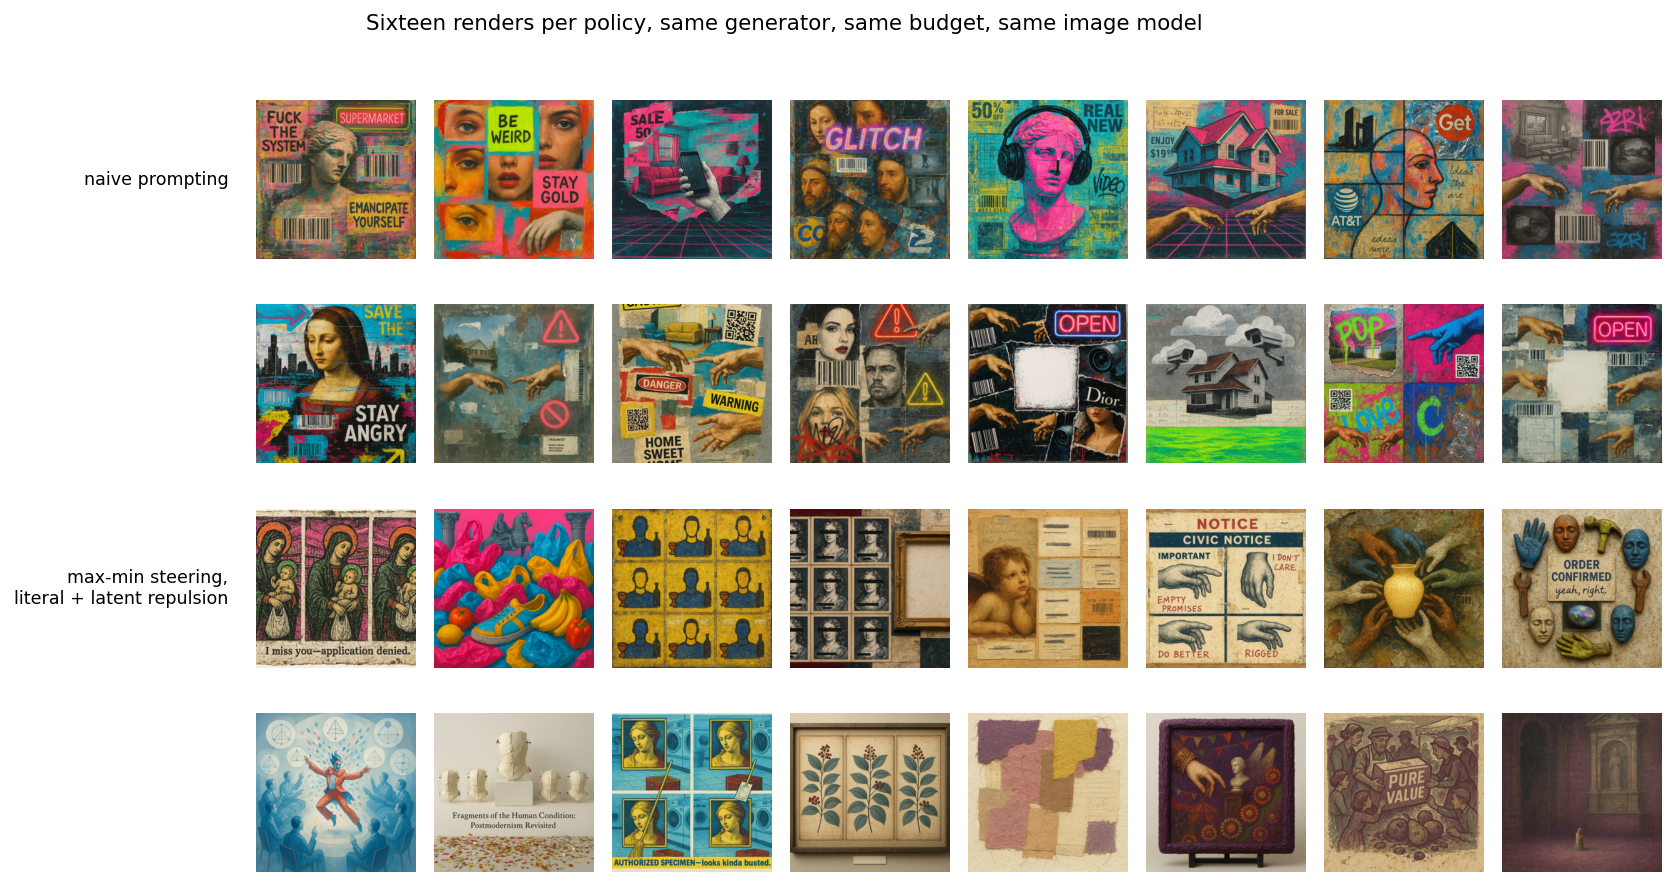
\includegraphics[keepaspectratio,alt={Figure 1. Sixteen renders per policy, same generator, same budget, same image model. Rows 1--2, naive prompting: a corpus with a 0.000 exact-duplicate rate and healthy lexical diversity that still returns one visual mode --- magenta and cyan collage, barcodes and QR codes, Renaissance portraits and classical busts, Michelangelo hands, warning triangles and neon OPEN signs recurring across nearly every panel. Rows 3--4, max-min steering with literal and latent repulsion on both the text and vision sides: medium, palette, register and composition all move, across a medieval triptych, a botanical cabinet, a photographed sculpture installation, a torn-paper abstract and a civic notice.}]{figures/fig13_contact_sheet.png}}

\emph{Figure 1. Sixteen renders per policy, same generator, same budget,
same image model. Rows 1--2, naive prompting: a corpus with a 0.000
exact-duplicate rate and healthy lexical diversity that still returns
one visual mode --- magenta and cyan collage, barcodes and QR codes,
Renaissance portraits and classical busts, Michelangelo hands, warning
triangles and neon OPEN signs recurring across nearly every panel. Rows
3--4, max-min steering with literal and latent repulsion on both the
text and vision sides: medium, palette, register and composition all
move, across a medieval triptych, a botanical cabinet, a photographed
sculpture installation, a torn-paper abstract and a civic notice.}

\subsubsection{5.3 Audio: whether a prompt can be steered is a property
of the
embedder}\label{53-audio-whether-a-prompt-can-be-steered-is-a-property-of-the-embedder}

The more portable finding is that whether a prompt can be steered before
rendering is a property of the \emph{embedder} rather than of music.
Measuring the Spearman correlation between prompt-pair similarity
through the text tower and track-pair similarity through the audio
tower:

{\footnotesize
\begin{longtable}[]{@{}>{\raggedright\arraybackslash}p{\dimexpr 0.3945\linewidth-2\tabcolsep\relax}>{\raggedright\arraybackslash}p{\dimexpr 0.2441\linewidth-2\tabcolsep\relax}>{\raggedright\arraybackslash}p{\dimexpr 0.3615\linewidth-2\tabcolsep\relax}@{}}
\toprule\noalign{}
embedder & alignment (naive / conditioned) & note \\
\midrule\noalign{}
\endhead
\bottomrule\noalign{}
\endlastfoot
\textbf{MuQ-MuLan} & \textbf{0.68 / 0.47} & a usable steering
gradient \\
CLAP-fused & 0.50 / 0.21 & weak; \textasciitilde0.05 on the steered
corpus \\
CLAP-music & 0.18 / 0.06 & worst; median within-corpus NN distance 0.004
--- it hears one track \\
\end{longtable}}

Cross-embedder agreement on pairwise track similarity spans 0.22--0.84,
per-arm diversity verdicts flip between embedders, and each embedder
nominates a different most-redundant pair. Two prescriptions follow:
steer music with MuQ-MuLan rather than CLAP, and never publish an
audio-diversity number without naming its embedder. Structural contracts
have a length ceiling as well --- compliance with a requested section
sequence is exact at prompt lengths near 560 characters, 0.11 at a mean
of 658, and zero by \textasciitilde1,600 --- so a structural contract
for music must be short or it is noise.

\subsubsection{5.4 The ranking does not depend on the
viewpoint}\label{54-the-ranking-does-not-depend-on-the-viewpoint}

A max-min score is a distance in a chosen embedding, so a natural worry
is that it names a property of the embedder rather than of the corpus.
Six exam-item corpora --- this method\textquotesingle s bank against
naive sampling, persona prompting, self-instruct, evol-instruct and
high-temperature sampling, 200 items each --- were scored under four
independent representations: CLIP text, TF-IDF with no learned semantics
at all, the twenty-two-feature prosodic vector, and a 150-dimensional
function-word profile of the kind used for authorship attribution. Each
score is the fifth-percentile nearest-neighbour distance divided by the
mean pairwise distance of the same cloud, which is invariant to the
global rescaling an embedding choice is free to apply, and each
representation is admitted only if its between-corpus spread exceeds its
own within-corpus sampling noise --- all four clear that bar by factors
of 9.7 to 24.7.

The four views agree, at a mean Kendall tau of +0.83 across their six
pairings, and \textbf{RAC ranks first under every one of them},
including the three it never optimizes. It also holds the best
worst-case score, so it wins under a distributionally-robust reading of
diversity as well as under any single view. The agreement is not an
artifact of the degenerate baselines: restricted to the three corpora
whose fifth-percentile distance is non-zero in every representation,
mean tau is +0.67 and RAC is still first under all four. Naive sampling
and high-temperature sampling score exactly zero on prosody and on
stylometry --- at least one item in twenty has an exact neighbour in
those channels.

\subsubsection{5.5 Literal and latent diversity move in opposite
directions}\label{55-literal-and-latent-diversity-move-in-opposite-directions}

Literal and latent diversity move in opposite directions in one corpus,
which is why both are reported throughout. Measuring the DALL·E naive
corpus as it grows:

{\footnotesize
\begin{longtable}[]{@{}>{\raggedright\arraybackslash}p{\dimexpr 0.3186\linewidth-2\tabcolsep\relax}>{\raggedright\arraybackslash}p{\dimexpr 0.1259\linewidth-2\tabcolsep\relax}>{\raggedright\arraybackslash}p{\dimexpr 0.1868\linewidth-2\tabcolsep\relax}>{\raggedright\arraybackslash}p{\dimexpr 0.1736\linewidth-2\tabcolsep\relax}>{\raggedright\arraybackslash}p{\dimexpr 0.1951\linewidth-2\tabcolsep\relax}@{}}
\toprule\noalign{}
\emph{n} & distinct-2 & 4-gram self-repetition & \emph{n}-gram Vendi &
centered embedding Vendi \\
\midrule\noalign{}
\endhead
\bottomrule\noalign{}
\endlastfoot
5 & 0.870 & 0.031 & 4.9 & 3.79 \\
40 & 0.492 & 0.211 & 30.2 & 24.13 \\
300 & 0.252 & 0.384 & 142.5 & 55.70 \\
1,000 & 0.145 & 0.520 & 246.6 & 63.05 \\
1,750 & 0.112 & 0.577 & 283.3 & 65.30 \\
\end{longtable}}

Literal diversity collapses monotonically --- by \emph{n} = 1,750 more
than half of each new instruction\textquotesingle s 4-grams have already
appeared --- while latent diversity rises and then saturates. Reporting
either alone supports an opposite conclusion about the same corpus.

\pandocbounded{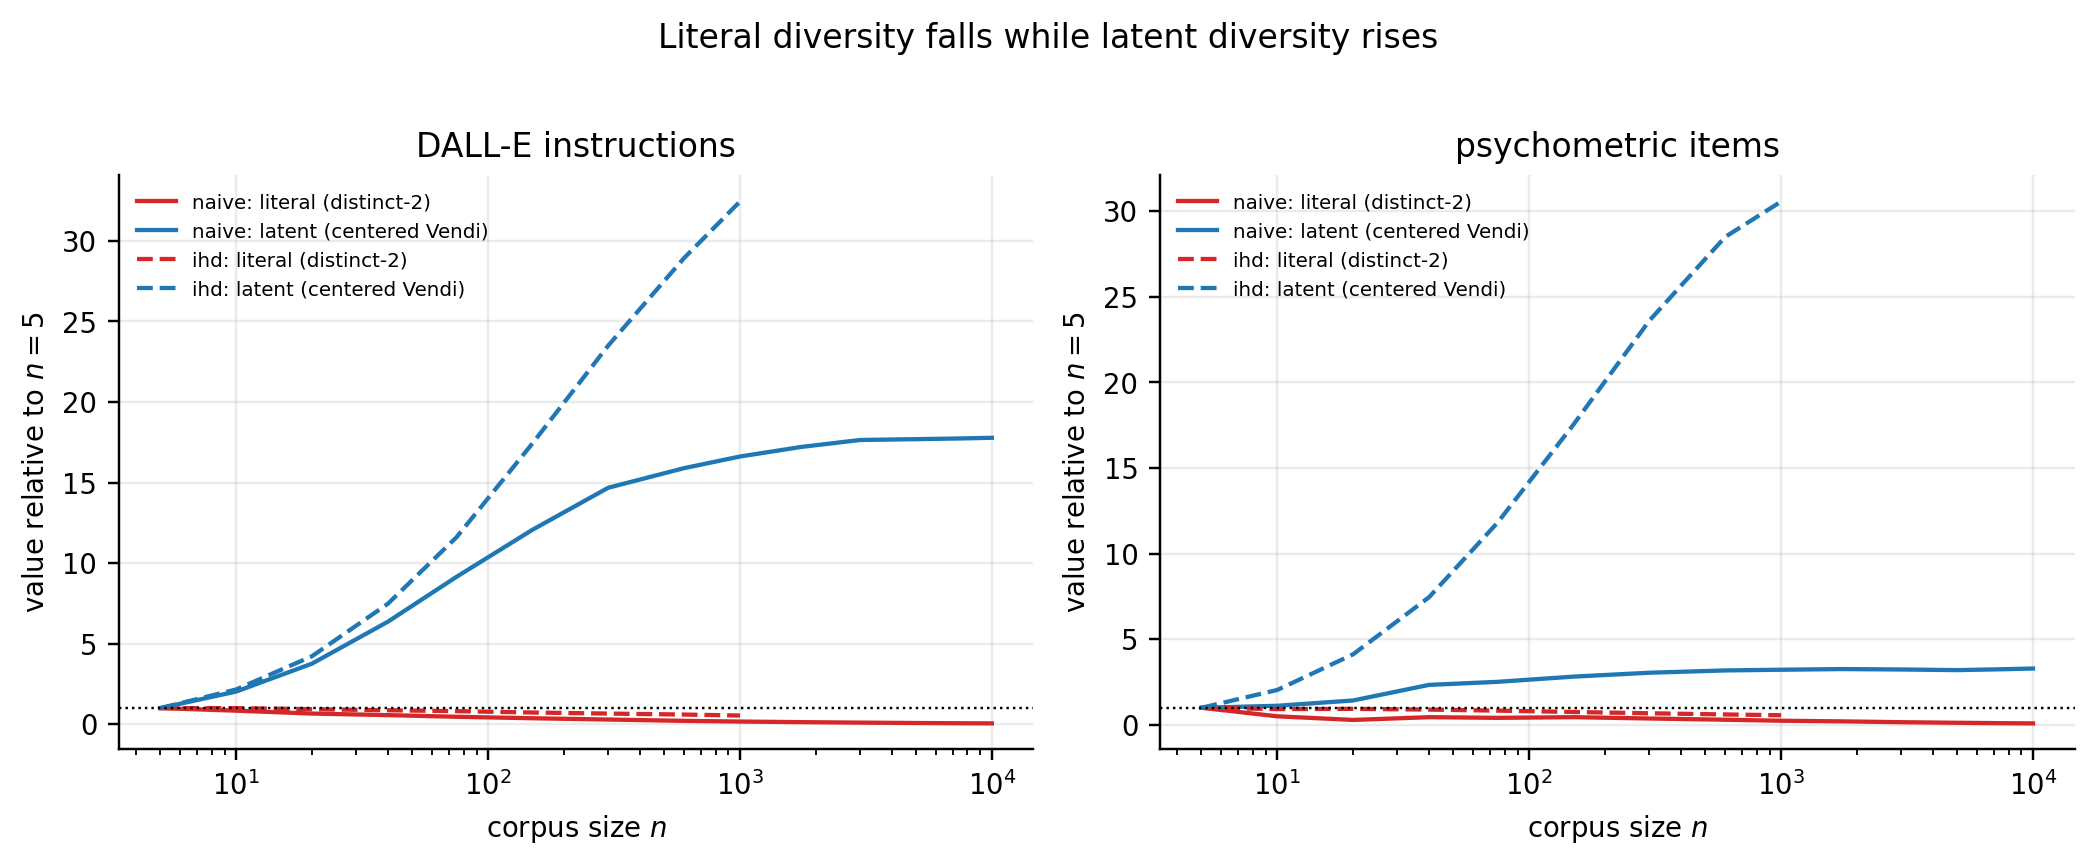
\includegraphics[keepaspectratio,alt={Figure 2. The decoupling, normalized to each series\textquotesingle{} value at n = 5. Literal diversity falls monotonically while latent diversity rises: two measurements of two different quantities that one word, "diversity", has been covering for.}]{figures/fig11_literal_vs_latent.png}}

\emph{Figure 2. The decoupling, normalized to each
series\textquotesingle{} value at n = 5. Literal diversity falls
monotonically while latent diversity rises: two measurements of two
different quantities that one word, "diversity", has been covering for.}

\subsubsection{5.6 A class of repetition the embedding
misses}\label{56-a-class-of-repetition-the-embedding-misses}

One comparison in the artifact channel runs against the method, and it
belongs here. Embedding metrics miss an entire class of visual
repetition --- tiled grids of one cell, a shared palette, the same
composition recoloured --- so we audit it with deliberately dumb
non-semantic signatures: a 16×16 luminance layout map, an
autocorrelation tiling score, a hue histogram. Scored at matched
\emph{n} = 60 and matched render tier, \textbf{the published baselines
are better than our arms on both structural measures}: layout twins
above 0.5 cosine average 0.223 across the five baselines against 0.473
across our eleven, and literal tilings 0.117 against 0.406, with no
baseline worse than our best arm on layout. A corpus told to differ
along seven or eleven named dimensions apparently converges on a
compositional template that plain repeated prompting does not. Adding
literal-space structural bans to the prompt --- grids banned when recent
renders tile, dominant hue pairs named and banned, layout-change demands
when layouts collide, plus a learned text→bad-structure bridge ---
halves palette twins (0.78 → 0.35 in the coverage arm) and improves the
coverage objective 21\% (0.206 → 0.247), but does not close it. Optical
spread and structural repetition are both measured on pixels and point
in opposite directions: our corpora occupy a wider region of that space
while repeating their compositional scaffolding more often within it.

\subsubsection{5.7 A defect no diversity measure can
see}\label{57-a-defect-no-diversity-measure-can-see}

The audits of §7 ask whether the axes reach the artifact. This one asks
whether the resulting bank is \emph{usable}. For a test bank, key
position is a hard requirement: correct answers must be distributed
across option positions, because an examinee who notices an imbalance
can exploit it without reading anything. Asking a fixed solver each item
and recording which position it chose:

{\footnotesize
\begin{longtable}[]{@{}>{\raggedright\arraybackslash}p{\dimexpr 0.3525\linewidth-2\tabcolsep\relax}>{\raggedright\arraybackslash}p{\dimexpr 0.1624\linewidth-2\tabcolsep\relax}>{\raggedright\arraybackslash}p{\dimexpr 0.0970\linewidth-2\tabcolsep\relax}>{\raggedright\arraybackslash}p{\dimexpr 0.0970\linewidth-2\tabcolsep\relax}>{\raggedright\arraybackslash}p{\dimexpr 0.0970\linewidth-2\tabcolsep\relax}>{\raggedright\arraybackslash}p{\dimexpr 0.1941\linewidth-2\tabcolsep\relax}@{}}
\toprule\noalign{}
bank & A & B & C & D & χ² vs uniform (3 df) \\
\midrule\noalign{}
\endhead
\bottomrule\noalign{}
\endlastfoot
RAC & \textbf{0.900} & 0.050 & 0.050 & 0.000 & \textbf{90.4} \\
naive & 0.225 & 0.550 & 0.225 & 0.000 & 24.6 \\
RAC, after balancing & 0.200 & 0.175 & 0.300 & 0.325 & \textbf{2.6} \\
\end{longtable}}

\textbf{Ninety percent of the RAC bank\textquotesingle s keys sit in
position A}, against a critical value of 7.81 at \emph{p} = .05. An
examinee who answers A to everything scores 90\% without reading a stem,
and neither bank ever places a key in D. This is a property of the
solver only if the solver is not reading the items, so we separated the
two by permutation: ask each item twice, once as written and once with
its options reordered, and record which option \emph{text} is chosen.
The answer follows the content in 95\% of RAC items and 100\% of naive
items, and stays on the same letter in only 17.5\% and 30\%. The solver
reads; the imbalance is in the bank.

\textbf{Why the method cannot see this.} Key position is not a semantic
property, so it is invisible to every measure in this paper ---
embedding diversity, \emph{n}-gram diversity, Vendi, coverage and the
enemy-item radius are all exactly as favourable on a bank whose key is
always A as on a balanced one. It is invisible to the axis set for the
same reason: all seven axes condition on item content, and even
\emph{distractor logic} governs what the distractors are like rather
than where the key sits among them. And it is structural rather than
accidental --- a generator asked for a stem and four options writes the
answer it has in mind first and builds distractors around it, so A is
where the key lands by default.

The repair needs no answer key. Permuting each item\textquotesingle s
options uniformly at random moves the key with its own text from
whatever position it held, so the bank becomes uniform by construction;
options whose text refers to a position ("none of the above", "both A
and B") are detected and left as written, which affects 37 of 1,999
items. Applied to the RAC bank this takes χ² from 90.4 to 2.6 ---
indistinguishable from uniform --- while content-tracking is unchanged
at 95\%.

The general form is the sharpest limitation in this paper. \textbf{A
diversity objective defined over an embedding is blind to any property
of the artifact the embedding does not encode, including properties that
decide whether the artifact can be used at all.} Difficulty is the same
story in the same domain: it is the parameter an item bank exists to
span, it is latent rather than semantic, and nothing in the objective
can see it. Measuring diversity well is not the same as measuring
fitness for purpose, and the gap between them is not visible from inside
the objective.

\subsection{6. Steering through the
proxy}\label{6-steering-through-the-proxy}

\subsubsection{6.1 Images: closing the loop where the product
lives}\label{61-images-closing-the-loop-where-the-product-lives}

The vision-steered arm closes the loop where the product lives. It
renders a bounded sample of accepted instructions, embeds them with
CLIP, and feeds two things back into the text-side loop: a least-squares
map from the crowded \emph{image} directions into instruction-embedding
space, so the text-side orthogonality term can push away from visual
redundancy it cannot itself perceive; and mined \emph{visual} attractors
from the vision judge, appended to the same ledger as the textual ones.
It is the paper\textquotesingle s mechanism applied one level down ---
the ledger already repels against what the model keeps saying, and now
also against what it keeps showing --- and it is the best arm in the
companion paper\textquotesingle s competitive comparison (its §7.2).

The margin is measurable in the space the loop optimizes and visible on
the page. At matched \emph{n} = 200 in the DALL·E domain, the text-only
RAC arm scores centered Vendi 77.67 and median nearest-neighbour
distance 0.171; the vision-steered arm scores 91.97 and 0.192, an 18\%
gain in centered Vendi, and leads every column of the seven-arm
comparison --- distinct-2 0.699 against 0.660, 4-gram self-repetition
0.040 against 0.068, \emph{n}-gram Vendi 170.9 against 167.0. The
contact sheet of §5.2 shows the same thing without a number: rows 3--4,
steered on both the text and the vision side, move medium, palette,
register and composition where rows 1--2 return one visual mode.

\subsubsection{6.2 Audio: cross-modal steering through an audio
embedder}\label{62-audio-cross-modal-steering-through-an-audio-embedder}

At matched \emph{n}, matched prompt length and the same generator, the
conditioned music arm reaches centered Vendi 43.03 against
naive\textquotesingle s 22.99 (1.87×), halves 4-gram self-repetition
(0.140 against 0.291), raises distinct-2 (0.545 against 0.348) and holds
roughly three times the room between nearest neighbours (0.079 against
0.027), on 100 prompts per arm with no exact duplicates in either --- so
the effect is semantic. On 100 rendered Lyria instrumentals generated by
cross-modal steering with zero rejection, 100\% of tracks verify as
instrumental in CLAP space and mean-centered CLAP Vendi is 17.43 against
11.5 for naive prompts and 14.1 for axis-conditioned prompts under the
same embedder.

The rendered arm was steered through CLAP and is measured in CLAP.
§5.3\textquotesingle s alignment table says the same loop through
MuQ-MuLan would have a steering gradient nearly four times as strong on
the naive arm (0.68 against 0.18), which is the experiment we would run
next; the prescription --- steer music with MuQ-MuLan rather than CLAP
--- is §5.3\textquotesingle s, and the loop is the image one of §6.1
with the audio tower in place of CLIP.

\subsubsection{\texorpdfstring{6.3 Best-of-\emph{K} at the render:
select on the channel the objective cannot
see}{6.3 Best-of-K at the render: select on the channel the objective cannot see}}\label{63-best-of-k-at-the-render-select-on-the-channel-the-objective-cannot-see}

The companion paper measures best-of-\emph{K} on the written candidate
(its §8.4): selecting on the gap alone raises the minimum
nearest-neighbour distance by 20\% in three of three seeds, at a cost of
a third of a craft point. The same question at the \emph{render} has a
sharper answer, because the two channels have very different effective
dimensions. Best-of-\emph{K} on the written candidate happens before the
handoff and §7 locates the loss after it, so we also ran \emph{K} = 3
renders behind each of 60 fixed instructions and kept the render
maximizing min distance to the accepted set --- once in CLIP, once in
optical statistics, over the same candidates. Selecting on optics raises
pixel min NN from 1.039 to 1.292 (1.24×) and the fifth-percentile NN by
0.336 (paired subsample, 95\% CI {[}+0.128, +0.488{]}), \textbf{and
costs nothing in the channel the method optimizes}: CLIP min NN moves by
−0.001 with the interval {[}−0.029, +0.033{]} tight around zero.
Selecting on CLIP raises CLIP min NN by 0.040 ({[}+0.025, +0.071{]}) and
moves optics not at all detectably. Both gains lie on the
\emph{K}\(^{1/m}\) curve --- 1.24× at \emph{K} = 3 implies \emph{m} ≈
4.4, and 1.04× implies \emph{m} ≈ 17 --- so render-side selection is
oversampling rather than a new mechanism. What the dimensions add is an
allocation rule: oversampling buys far more in a low-dimensional channel
than in a high-dimensional one, and \textbf{if a pipeline is going to
pay for extra renders, it should select them on the channel the
objective cannot see.}

\subsection{7. Conditioning across the
seam}\label{7-conditioning-across-the-seam}

The companion paper audits whether a commanded axis level shows up in
the artifact (its §8.1), by manipulation rather than correlation: hold a
base spec fixed, set one axis to each of its levels in turn, generate,
and read the displacement, centring within base so that only variation
produced by \emph{setting} the axis contributes, with a null that
shuffles levels within each base. Two instruments read each artifact ---
\emph{identifiability}, whether CLIP(ℓ) is the nearest of the
axis\textquotesingle s level descriptions to an image generated under
level ℓ, against a chance rate of 1/\textbar levels\textbar; and
\emph{separation}, the η² of artifact embeddings grouped by commanded
level under a permutation null --- and a third channel that lives
outside the embedding the method optimizes: pixel statistics for images,
prosody for poems. On poems every axis is realized on at least one
channel. On images three of seven axes identify their level at or below
chance, two are undetectable on both channels, and the axis the
attribution scoring ranked \emph{first} is the least realized in the
corpus. The image domain is where the proxy question becomes a
conditioning question, because the image pipeline has a seam the poem
pipeline does not.

\pandocbounded{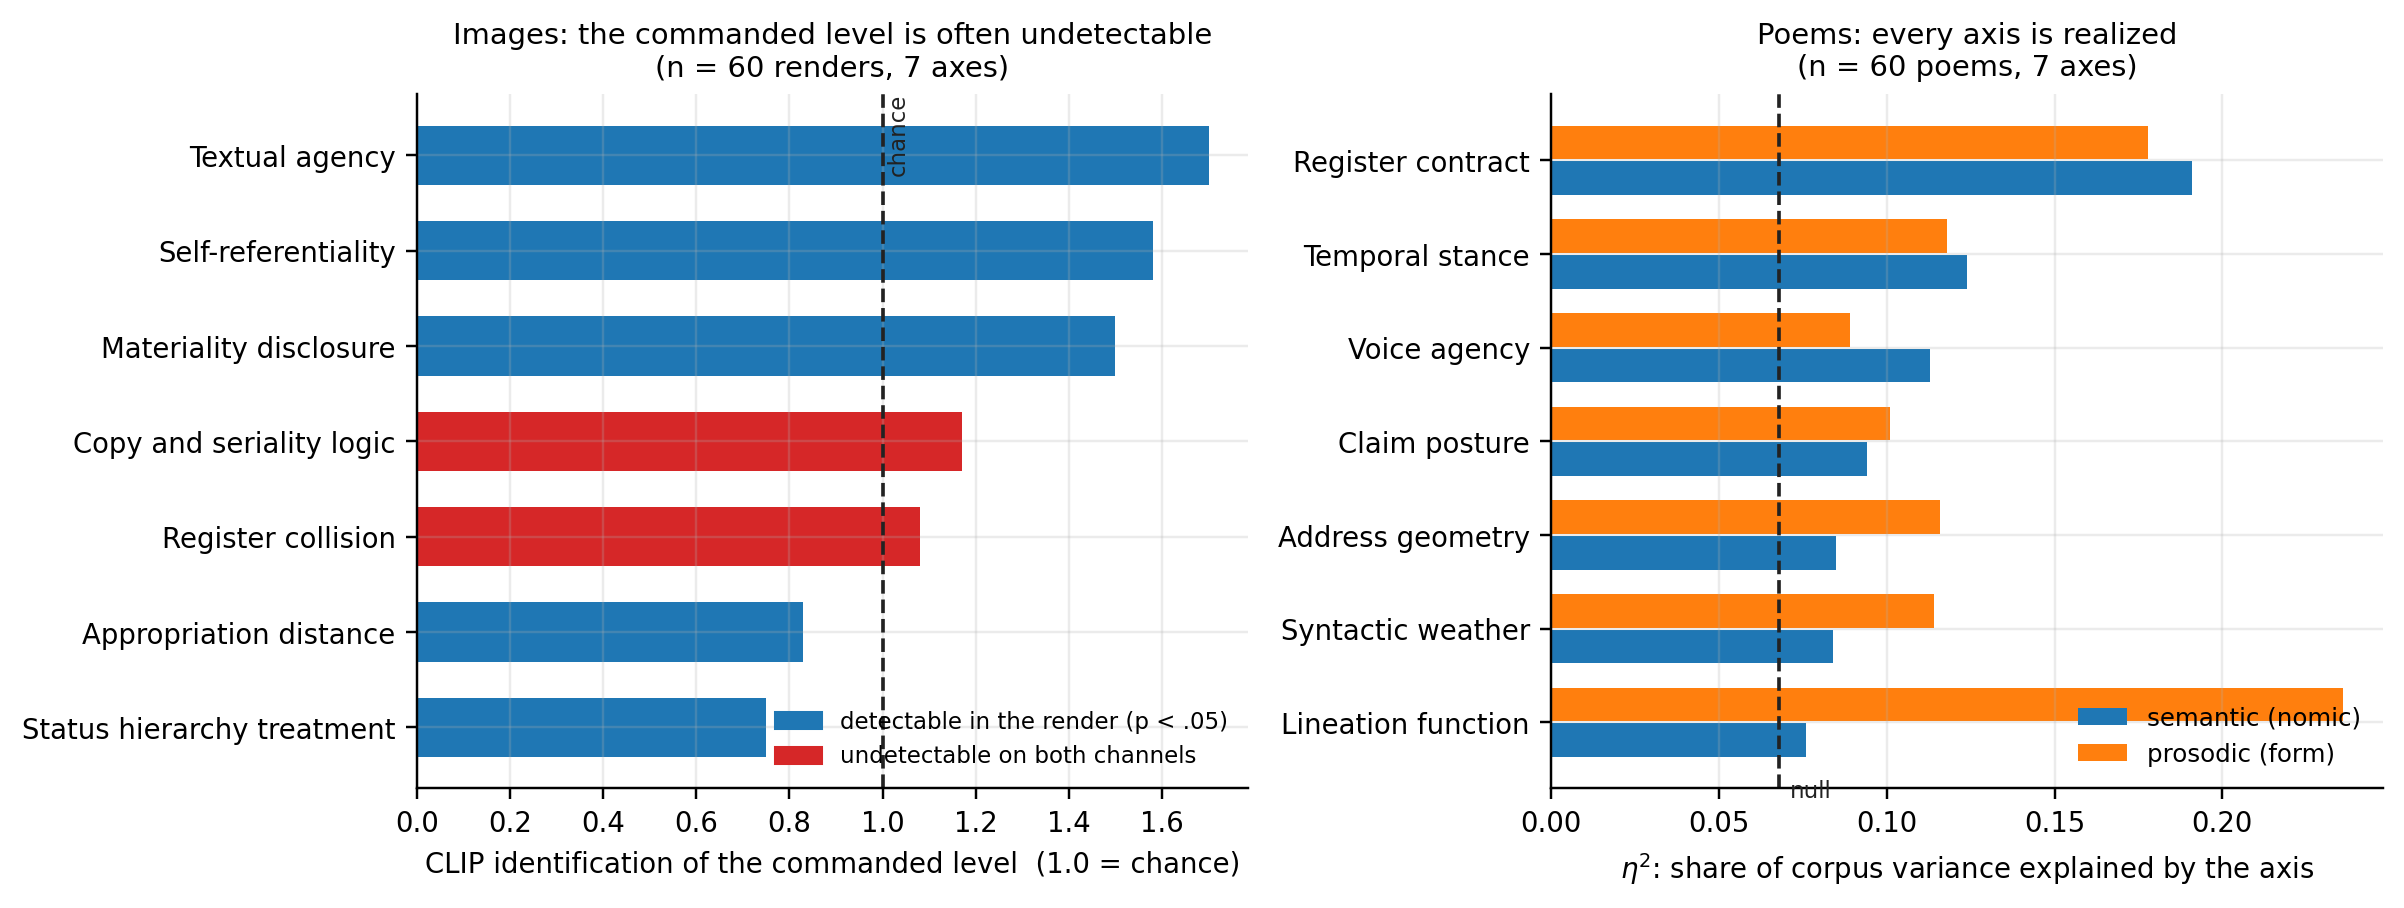
\includegraphics[keepaspectratio,alt={Figure 3. Axis realization measured on the artifact. Left: on 60 max-min renders, three of seven axes identify their commanded level at or below chance, and two are undetectable on both the CLIP and pixel channels. Right: on 60 poems, every axis is realized --- on the semantic channel, the prosodic channel, or both. Dashed lines mark chance and the permutation null.}]{figures/fig17_axis_realization.png}}

\emph{Figure 3. Axis realization measured on the artifact. Left: on 60
max-min renders, three of seven axes identify their commanded level at
or below chance, and two are undetectable on both the CLIP and pixel
channels. Right: on 60 poems, every axis is realized --- on the semantic
channel, the prosodic channel, or both. Dashed lines mark chance and the
permutation null.} \textbf{Images, by intervention: the loss is at the
render, not in the writing.} The image pipeline has two stages --- the
model that proposed the axes writes an instruction, and
\texttt{gpt-image-1-mini} renders it --- so the same manipulation can be
read on both sides of the handoff. Over all eleven axes at three bases
and five levels, embedding the written instruction with CLIP, the render
with CLIP, and the render\textquotesingle s optics separately: nine of
eleven axes are realized in the \textbf{written instruction} at \emph{p}
\textless{} 0.05 (mean ρ = 0.148), against four of eleven in the
\textbf{render} (mean ρ = 0.096). Ten of the eleven attenuate, a mean
loss of 35\% of the text-side effect (Wilcoxon signed-rank \emph{p} =
.005; paired \emph{t}, \emph{p} = .003, both two-sided).
\textbf{Conditioning reaches the instruction and loses a third of its
grip at the render.} The image domain\textquotesingle s weak realization
is therefore not a failure of the axis calculus to produce usable
conditioning --- the conditioning is there, in the prompt, and
measurable --- but of that conditioning to survive a generator that
never saw the axis set.

Part of the apparent loss is the instrument rather than the renderer,
and this is the §5.1 lesson arriving from the other direction. The four
perceptual axes attenuate most in CLIP and are precisely the axes CLIP
is least equipped to register: measured on pixels instead,
\emph{Lighting direction} reads 0.229 against 0.092 in CLIP, \emph{Shot
scale} 0.252 against 0.105, and \emph{Motion and temporal blur} 0.203
against 0.069. An axis commanding optics moves the optics and barely
moves a semantic embedding.

\textbf{The seam explains the split.} The calculus is identical across
the two domains, the axes are comparably abstract, and the budgets
match. What differs is where the conditioning has to travel. A poem is
written by the same model that proposed the axes, so the conditioning
never leaves the system that understands it. An image axis is written by
that model into a prompt and handed to a different model, which never
saw the axis set, shares no latent space with it, and is under no
obligation to honour a distinction like \emph{copies outrank an absent
original}. §5.2 measured this seam from the outside as a proxy gap; the
intervention measures it from the inside. \textbf{Conditioning strength
degrades at the boundary where the generator changes hands}, so the
modality-agnostic claim holds for the calculus --- which needs only an
embedding --- and not for the conditioning, which needs a generator that
reads the same language the axes are written in.

\subsection{8. Scoring axes in the artifact\textquotesingle s
space}\label{8-scoring-axes-in-the-artifacts-space}

The companion paper scores a candidate axis by four factors --- spread,
transversality, independence and headroom (its §5.2) --- all computed
from \emph{level vectors}: one embedding per level of each axis. In the
text-only setting those are embeddings of the level descriptions ---
what a level \emph{claims} it will do. Once the artifact can be
embedded, the natural improvement is to replace them with the centroid
of everything actually produced under each level: what the level
\emph{did}. That substitution is what makes the scoring empirical, and
on its own it is wrong.

A centroid computed that way is a \textbf{marginal mean where the score
needs a partial effect}. Specs are sampled independently, so every other
axis varies inside each level group; with sixty items, seven axes and
five levels each, a group holds about twelve items whose spread is
mostly produced by the other six axes. The estimator cannot tell "this
axis moves the artifact" from "this axis co-occurred with movement", and
nothing in the loop ever intervenes on one axis while holding the rest
fixed.

The consequence is not a modest loss of precision. It is a
\textbf{systematic inversion}, and the mechanism is our own
transversality term. An axis that genuinely moves the artifact fills the
corpus with variance along its own direction; the occupied eigenspace
absorbs that direction; and transversality --- the fraction of an
axis\textquotesingle s variation lying \emph{outside} the occupied span
--- collapses toward zero for precisely that axis. An axis the generator
ignores contributes only isotropic noise, little of which the occupied
basis captures, so its transversality stays high. Because promise is
multiplicative, the effective axis sinks and the inert one rises.
\textbf{The better an axis is, the harder the score punishes it.} The
repair --- partial effects from one additive model over all axes, a
null-corrected realization factor ρ, and the interventional probe when a
generation budget can be spent on measurement --- is the companion
paper\textquotesingle s §5.3, and it is what makes artifact-space
scoring usable: with it the strong axis ranks first on all 24 seeds of a
ground-truth test where the attribution form ranked the inert axis first
in 17 of 24. What belongs here is the consequence for a proxy. Level
vectors read in the artifact\textquotesingle s own embedding are only as
good as that embedding\textquotesingle s grip on the axis. §7 shows the
four perceptual image axes attenuate most in CLIP and are precisely the
axes CLIP is least equipped to register --- \emph{Lighting direction}
reads 0.229 on pixels against 0.092 in CLIP --- so an axis commanding
optics can be scored as inert in the very space that was adopted to make
the scoring honest. Where a designed feature channel exists for the
artifact, the realization factor should be computed there as well, and
the axis kept if either channel finds it.

\subsection{9. Decode instead: the oracle is usually cheaper than the
proxy}\label{9-decode-instead-the-oracle-is-usually-cheaper-than-the-proxy}

The argument for computing distances on text rather than on the artifact
is always the same, and it is never stated as an argument because it is
assumed: decoding is expensive, embedding is cheap, so one embeds. For a
rendered image or a two-minute instrumental that is true. For the
decoders in this section it is false, and by a wide margin.

Measured on one laptop, per item:

{\footnotesize
\begin{longtable}[]{@{}>{\raggedright\arraybackslash}p{\dimexpr 0.6300\linewidth-2\tabcolsep\relax}>{\raggedright\arraybackslash}p{\dimexpr 0.2074\linewidth-2\tabcolsep\relax}>{\raggedright\arraybackslash}p{\dimexpr 0.1627\linewidth-2\tabcolsep\relax}@{}}
\toprule\noalign{}
operation & ms per item & relative \\
\midrule\noalign{}
\endhead
\bottomrule\noalign{}
\endlastfoot
decode: string → \texttt{ipaddress} arcs, plain execution &
\textbf{0.11} & 1× \\
decode: same, with \texttt{sys.settrace} instrumentation & \textbf{0.98}
& 9× \\
decode: Python program → 140-input battery, \textbf{each in a fresh OS
process} & \textbf{29.1} & 265× \\
embed: \texttt{nomic-embed-text}, local Ollama, batched & 107.9 &
981× \\
embed: \texttt{nomic-embed-text}, local Ollama, one at a time & 1,488.2
& 13,529× \\
embed: character TF-IDF, local, batched & 18.3 & 166× \\
\end{longtable}}

The code row is deliberately the least favourable decode measurement we
can honestly make: every generated program is run in a \emph{separate
operating-system process} for isolation, so Python interpreter start-up
dominates and the actual execution is a rounding error. Even so,
decoding is \textbf{3.7× cheaper than a batched local embedding} and
\textbf{51× cheaper than embedding items one at a time}, which is what a
streaming pipeline does. Where the decoder does not need process
isolation the margin is three orders of magnitude.

Two honest qualifications. Instrumentation, not the program, is the
dominant decode cost --- tracing costs 9× plain execution --- so a
decoder whose instrumentation is heavy needs its own measurement rather
than an inherited ratio. And the embedding figures are for a
\emph{local} model with no network hop and no per-token charge, which is
the best case for the text-space route; a hosted embedding endpoint is
slower and has a price.

The conclusion is not rhetorical. \textbf{For a deterministic decoder
that runs in milliseconds, the artifact-space oracle is not the
expensive option a practitioner forgoes. It is the cheap option they did
not think to run}, and it recovers between 1.02× and 1.64× the coverage
of the best text-space selector at matched budget (§4.6), reaching at
\emph{k} = 30 what text-space selection needs \emph{k} = 100 to reach.

Where decoding genuinely is expensive --- rendered images, audio,
anything behind a paid endpoint --- the fallback is not a text-space
selector but a \emph{partial decode budget}: decode a sample, and spend
the rest of the budget where the sample says the behaviour is. That
regime is where §6\textquotesingle s cross-modal steering belongs, and
it is the boundary between the two halves of this paper.

\subsection{\texorpdfstring{10. \texttt{decodergap}: the
probe}{10. decodergap: the probe}}\label{10-decodergap-the-probe}

The results above do not compose into a rule a practitioner can apply
blind, because the one decision whose sign varies --- far-field
selection --- varies \emph{by decoder}, and nothing visible in the text
says which case you are in. What they compose into is a measurement, and
the measurement is cheap enough to run before any pipeline decision is
committed.

\texttt{decodergap} takes three things: a corpus, an embedding function,
and a decode function returning anything with a distance on it. It
returns the near-field profile, the two deduplication verdicts, and the
selector comparison against the artifact-space oracle.

\begin{Shaded}
\begin{Highlighting}[]
\ImportTok{from}\NormalTok{ decodergap }\ImportTok{import}\NormalTok{ probe}

\NormalTok{report }\OperatorTok{=}\NormalTok{ probe(}
\NormalTok{    texts     }\OperatorTok{=}\NormalTok{ corpus,                    }\CommentTok{\# what you generated}
\NormalTok{    embed     }\OperatorTok{=}\NormalTok{ my\_embedder,               }\CommentTok{\# what you were going to select in}
\NormalTok{    decode    }\OperatorTok{=} \KeywordTok{lambda}\NormalTok{ s: run(s, battery), }\CommentTok{\# what the item actually becomes}
\NormalTok{    distance  }\OperatorTok{=}\NormalTok{ jaccard,                   }\CommentTok{\# a distance on the decoded artifact}
\NormalTok{    coverage  }\OperatorTok{=}\NormalTok{ distinct\_cells,            }\CommentTok{\# what a subset is meant to buy}
\NormalTok{)}
\NormalTok{report.verdicts[}\StringTok{"deduplication\_aggregate"}\NormalTok{]   }\CommentTok{\# SUPPORTED | UNSUPPORTED}
\NormalTok{report.verdicts[}\StringTok{"deduplication\_per\_item"}\NormalTok{]    }\CommentTok{\# SUPPORTED | NOT SUPPORTED}
\NormalTok{report.verdicts[}\StringTok{"max\_min\_selection"}\NormalTok{]         }\CommentTok{\# SAFE | UNSAFE, and vs the oracle}
\end{Highlighting}
\end{Shaded}

Three design decisions carry the tool, and each is a finding from above
rather than a preference.

\textbf{It never reports a correlation without its decoder-free
control.} The profile of §4.2 looks like a finding and is reproduced
twice as strongly by two encoders that never saw a program run (§4.3).
Any proxy-qualification number the tool emits is accompanied by the
encoder-to-encoder baseline it has to beat, and by the permutation null
that shows whether any association exists at all.

\textbf{It issues two deduplication verdicts, not one.} The aggregate
verdict answers \emph{can this radius rank duplicate pairs at all}; the
per-item verdict answers \emph{of the pairs a filter at this radius
would reject, how many are behaviourally far apart}. On both decoders
measured here the first passes and the second fails, at 45.4\% and
41.6\%. A tool that emitted a single "dedup: safe" would be licensing
the decision its own data refuses.

\textbf{It scores every selector in the artifact\textquotesingle s space
and against the oracle}, so a text-space selector cannot win by agreeing
with the representation it selected in, and beating random is not
mistaken for doing well.

It also refuses to recommend a filter radius. We swept the threshold
over the 5th to 40th percentiles of each corpus\textquotesingle s own
distance distribution at four budgets: the best cell on the
\texttt{ipaddress} decoder is +20.7 arcs over random at \emph{t} = 10th
percentile and \emph{k} = 10, and by \emph{k} = 50 every threshold
loses. Any single-budget experiment would have produced a
shippable-looking constant. The sweep is reported in full, including the
cells that lose, and no constant is offered.

\subsection{11. Practice}\label{11-practice}

The prescriptions are short, and each is attached to the measurement
that motivates it. The first four are the ones we would keep if we could
keep four.

\begin{enumerate}
\def\labelenumi{\arabic{enumi}.}
\tightlist
\item
  \textbf{Never report a proxy-validation correlation without a
  decoder-free control.} Correlate your embedding against a second,
  unrelated representation of the same corpus, and against a permuted
  version of your artifact measurement. Whatever agreement survives
  above the first is what the artifact contributed; the second tells you
  whether any association exists. On our corpus the encoder-to-encoder
  baseline was \textbf{twice} the decoder signal (§4.3), which retires
  the finding we had.
\item
  \textbf{Qualify a proxy by running the decision, not by correlating
  the distances.} A correlation summarizes a geometry and inherits that
  geometry\textquotesingle s confounds. A decision is scored in the
  artifact\textquotesingle s space and either works or does not: what
  fraction of the pairs your filter drops are genuinely duplicates, how
  much artifact coverage your selector buys against the oracle.
\item
  \textbf{Split every deduplication claim into a corpus claim and an
  item claim.} They have different evidence and on both decoders here
  they get different verdicts: AUC 0.779 for ranking duplicate pairs,
  and 45.4\% of rejected pairs behaviourally far apart at the tightest
  radius (§4.5). Contamination screening is defensible; a per-item gate
  is not.
\item
  \textbf{If your decoder is deterministic and fast, do not select in
  text space at all.} Decoding cost 29.1 ms per item against 107.9 ms to
  embed one, in the least favourable measurement we could construct
  (§9), and the artifact-space oracle reached at \emph{k} = 30 what
  text-space selection needed \emph{k} = 100 to reach (§4.6). The oracle
  is the cheap option, not the expensive one.
\item
  \textbf{Name the embedder, and publish the pairwise-similarity
  distribution it operates on.} Per-arm audio verdicts flip between
  embedders and each nominates a different most-redundant pair (§5.3);
  mean pairwise cosine was 0.883 in one text corpus and 0.444 in another
  under the same embedder. A diversity number without its embedder and
  its similarity distribution is not a number.
\item
  \textbf{Count exact duplicates before computing anything, and report
  the literal and the latent separately.} They move in opposite
  directions in the same corpus (§5.5), and a 74\% duplicate rate makes
  every distance statistic a statistic about duplication.
\item
  \textbf{Measure at the level of the artifact you ship.} Text-embedding
  similarity explains 14.5\% of the variance in whether rendered images
  look alike, pooled across seven arms, and 8.2\% within-arm (§5.2). If
  the artifact is rendered, the objective belongs in the space the
  artifact occupies.
\item
  \textbf{Audit in at least one channel the objective never optimizes},
  with a distance statistic rather than a spectral one (§5.1). It is the
  only measurement that cannot be a restatement of the selection rule,
  and it is where the strongest positive result and the largest
  undetected defect in this line of work were both found.
\item
  \textbf{When a render is in the loop, steer through it.} Render a
  bounded sample, embed it in the artifact\textquotesingle s space, and
  bridge its crowded directions back into the text space the loop
  optimizes (§6.1); steer audio through an embedder whose text and audio
  towers agree (§6.2).
\item
  \textbf{Spend extra renders on the low-dimensional channel.}
  Best-of-\emph{K} buys \emph{K}\(^{1/m}\); selecting renders on nine
  pixel statistics buys 1.24× at \emph{K} = 3 where selecting on CLIP
  buys 1.04× (§6.3).
\item
  \textbf{Measure axis realization at the artifact, by intervention,
  wherever the generator changes hands} (§7). Where the seam exists, a
  third of the conditioning does not cross it.
\item
  \textbf{Balance by construction what the embedding cannot see.} Key
  position, difficulty, compositional template: none is encoded, none is
  optimized, and each decides usability. A uniform permutation of
  options needs no answer key and takes χ² from 90.4 to 2.6 (§5.7); a
  structural ban block halves palette twins (§5.6).
\item
  \textbf{Read the output.} A corpus can be diverse along every
  dimension you thought to measure and uniform along the one you did
  not.
\end{enumerate}

\subsection{12. Limitations}\label{12-limitations}

\begin{itemize}
\tightlist
\item
  \textbf{One text embedder.} All text geometry is
  \texttt{nomic-embed-text} with cosine distance. §5.4 shows the
  \emph{ranking} of methods survives four representations; whether the
  \emph{magnitudes} transfer is untested, and the companion
  paper\textquotesingle s coverage and packing numbers inherit that.
\item
  \textbf{A joint embedder varies both towers at once.} §5.3 changes one
  knob --- the model supplying both the text tower and the audio tower
  --- so it shows that the alignment moves and cannot say which side
  moves it. Crossing text-side and artifact-side encoders independently
  on fixed bytes is the decomposition this paper does not contain.
\item
  \textbf{The renders carry no logged seed.} The image endpoint exposes
  no seed parameter, so no render in this paper can be regenerated, and
  render stochasticity cannot be separated from the quantity being
  measured. Every artifact-space number here --- the proxy correlations
  of §5.2, the realization of §7, the render selection of §6.3 --- is a
  statement about an unlogged seed distribution, and a repeat-draw floor
  at a logged seed is the missing measurement.
\item
  \textbf{Several image results are single-seed.} The image arms are one
  seed each at \emph{n} = 60; the vision-steered arm\textquotesingle s
  margin in §6.1 is one run at \emph{n} = 200; the audio steering arm is
  one run of 100 tracks.
\item
  \textbf{Judge bias is unmeasured.} Vision and language-model judges
  name attractors, classify blueprint areas and read device forms; none
  is calibrated against human raters, and a judge that shares the
  generator\textquotesingle s blind spots would miss exactly what the
  generator misses.
\item
  \textbf{The structural signatures are deliberately dumb.} A 16×16
  luminance map, a tiling score and a hue histogram find tilings and
  palette twins and nothing subtler; they are a floor on what the
  embedding misses, not a measure of it.
\item
  \textbf{Steering closes part of the gap and not all of it.}
  Literal-space bans halve palette twins and improve the coverage
  objective by 21\% and do not close the structural deficit; the
  vision-steered arm is the best arm in the image domain and still
  renders through a model that never saw the axes.
\end{itemize}

\subsection{13. Conclusion}\label{13-conclusion}

An embedding oracle is the only thing the loop can see, and it is always
a proxy. In the two domains where the artifact is rendered by a model
the embedder never meets, the proxy explains a seventh of the variance
in what the reader receives, whether a prompt can be steered at all
depends on which embedder is asked, and a third of the conditioning does
not survive the handoff. In the domains where the artifact is text, the
embedding is still blind to metre, to compositional template, and to
where an answer key sits --- properties that decide whether the corpus
can be used.

None of this is an argument against the method; it is an argument about
where the method\textquotesingle s numbers are true. The extension that
follows is to treat the proxy as a proxy: render a sample and steer
through the artifact\textquotesingle s own space, spend oversampling
budget on the channel the objective cannot see, audit realization by
intervention at the seam, and balance by construction what no embedding
encodes. Under those rules the ranking the companion paper reports is
robust --- first under four representations, three of which the method
never optimized, at a mean Kendall τ of +0.83 --- and the gap between a
diverse corpus and a usable one is at least visible, which is the
precondition for closing it.

\end{document}
